%% Elsevier CAS conversion of manuscripts/trans/main_trans.tex.
%% Build from this directory with: pdflatex main_cas.tex

\documentclass[a4paper,fleqn]{cas-sc}

\usepackage[numbers]{natbib}
\usepackage{amsmath,amssymb}
\usepackage{booktabs}
\usepackage{multirow}
\usepackage{subcaption}
\usepackage{xcolor}
\usepackage{float}
\usepackage{placeins}

\graphicspath{{./images/}}
\emergencystretch=2em

\providecommand{\figref}[1]{\hyperref[#1]{Fig.~\ref*{#1}}}
\providecommand{\figsubref}[2]{\hyperref[#1]{Fig.~\ref*{#1}.#2}}
\renewcommand{\tabref}[1]{\hyperref[#1]{Table~\ref*{#1}}}

\begin{document}
\let\WriteBookmarks\relax
\def\floatpagepagefraction{1}
\def\textpagefraction{.001}

\shorttitle{Privacy-Preserving Interpretable Single-Domain Generalization}
\shortauthors{Q. Jin et~al.}

\title[mode=title]{Privacy-Preserving Interpretable Single-Domain Generalization for Multi-Label Ocular Disease Recognition}

\author[1]{Qiang Jin}

\author[1]{Xinyi Liu}

\author[1]{Li Yi}

\author[2]{Tian-Tian Zhang}

\author[3]{Yanhua Chen}

\author[1]{Zhi-Ri Tang}[orcid=0000-0002-0900-6500]
\cormark[1]
\ead{tangzhiri@jnu.edu.cn}

\author[4]{Rammohan Mallipeddi}

\affiliation[1]{organization={School of Intelligent Systems Science and Engineering/JNU-Industry School of Artificial Intelligence, Jinan University},
                country={China}}

\affiliation[2]{organization={Department of Electronic Engineering and Computer Science, Hong Kong Metropolitan University},
                city={Hong Kong},
                country={Hong Kong}}

\affiliation[3]{organization={Division of Science, Engineering and Health Studies, School of Professional Education and Executive Development, The Hong Kong Polytechnic University},
                city={Hong Kong},
                country={Hong Kong}}

\affiliation[4]{organization={Department of Artificial Intelligence, School of Electronics Engineering, Kyungpook National University},
                city={Daegu},
                country={Republic of Korea}}

\cortext[cor1]{Corresponding author: Prof. Zhi-Ri Tang}

\begin{abstract}
Early fundus screening is effective for ocular disease diagnosis. Deep learning has provided tools for fundus image analysis. However, clinical deployment still faces three major challenges: (1) multiple diseases often co-occur in a single eye, causing false positives and false negatives when modeled independently; (2) cross-institutional deployment suffers from domain shift, yet conventional cross-domain methods typically require target-domain or multi-source data, often infeasible; (3) medical data are privacy-sensitive, further restricting cross-institutional sharing and invalidating the multi-source assumption, calling for generalization with local privacy preservation. To address these three challenges in order, we first propose an Adaptive Label-Feature Relevance Construction (ARC) module that captures disease co-occurrence dependencies via Transformer attention to reduce false positives and negatives. Then, we design a Dual-Branch Guided Domain-Invariant Feature Extraction (DFE) module that learns domain-invariant features from a single source domain under Class Activation Mapping (CAM) guidance, improving unseen-domain generalization and interpretability. Finally, we integrate an Adaptive Gaussian Differential Privacy (AdaGDP) mechanism into training, preserving privacy through dynamic gradient noise injection with controlled performance loss. Experiments show that our method reaches a Final score of 78.85 on ODIR, outperforming representative multi-label ocular disease recognition methods, and yields a 3.19-point gain on EDID. Overall, we establish an interpretable and privacy-preserving single-domain generalization framework for multi-label ocular disease recognition, improving cross-domain performance and providing insights into ocular diagnosis under privacy constraints.
\end{abstract}

\begin{highlights}
\item Models label-feature disease relevance with Transformer-based attention.
\item Learns CAM-guided domain-invariant features from a single source domain.
\item Balances privacy and generalization via adaptive Gaussian gradient noise.
\end{highlights}

\begin{keywords}
Domain Generalization \sep Multi-Label Ocular Disease Recognition \sep Data Privacy \sep Interpretability
\end{keywords}

\maketitle


\section{Introduction}

Early fundus screening is an effective approach for ocular disease diagnosis, as it can reveal diverse pathological signs in the retina, optic disc, blood vessels, and macular region. Analyzing fundus images helps identify potential lesions and supports early intervention, thereby reducing the risk of irreversible visual impairment or even vision loss. As fundus screening continues to expand, manual fundus screening is limited by its time cost, dependence on expert experience, and shortage of primary medical resources. Fundus-image-based ocular disease diagnosis therefore has important practical value \cite{_Ref213949315}. Existing methods for fundus screening can be broadly grouped into three technical directions: Machine Learning (ML), Vision-Language Model (VLM), and Convolutional Neural Network (CNN). ML methods usually rely on hand-crafted features such as image enhancement, lesion segmentation, texture, or morphology, followed by classifiers such as support vector machines or random forests for recognition \cite{_RefRahman2022MLFundus}. These methods offer a degree of interpretability, but their feature design depends heavily on prior experience and has limited capacity to represent complex fundus lesions and multi-disease co-occurrence. In recent years, VLM has opened new directions for fundus image understanding, image-text joint analysis, and medical report generation \cite{_RefLim2024VLVOphthalmology} \cite{_RefUrooj2025LLMMedicalImage}. However, their training and fine-tuning generally require large-scale high-quality annotations, paired image-text data, and substantial computational resources, which remain costly when medical data are scarce, privacy is restricted, and clinical deployment resources are limited. In contrast, CNN-based deep visual models can directly learn local textures, lesion regions, and spatial structural features from fundus images, and have been widely applied to disease recognition \cite{_Ref213871637}, lesion segmentation \cite{_Ref213948625}, medical image reconstruction \cite{_Ref213948898}, and diagnosis and prediction of ocular diseases \cite{_Ref213949262}. Therefore, we adopt CNN as the main modeling backbone for multi-label ocular disease recognition. Nevertheless, in real-world clinical deployment, CNN-based ocular disease recognition methods still face challenges including multi-disease co-occurrence, degraded generalization performance across institutions, and privacy preservation. Specifically:

1. In clinical ocular disease diagnosis, a single eye may present multiple diseases simultaneously. Using a standard single-label classifier, or modeling different diseases as fully independent, can therefore lead to false positives and false negatives \cite{_Ref213949362}. Multi-label recognition has also been widely studied for natural images. For example, ML-GCN \cite{_Ref213949382} constructs graph relevance from label co-occurrence frequencies, making relevant labels more likely to be recognized once a given label is identified and thereby reducing false negatives. However, in multi-label ocular disease recognition, disease relevance is more complex, and methods that infer disease relevance solely from label co-occurrence frequencies may be insufficiently reliable. For multi-disease co-occurrence in fundus images, a more reliable method for label-feature relevance construction is therefore needed.

2. Medical images differ from natural images because their annotations usually require professional physicians, making both data acquisition and annotation costly. In addition, data sharing restrictions and inconsistent label spaces across medical institutions often limit access to multi-source-domain data and collaborative training. Even when a model performs well on the training set of one medical institution, applying it to another institution can introduce domain shift in the target domain because of differences in imaging devices, illumination conditions, and manual processing procedures \cite{_Ref213949348}, resulting in performance degradation. As shown in \hyperref[fig:intro-domain-gap]{Fig.~\ref*{fig:intro-domain-gap}.a1} and \hyperref[fig:intro-domain-gap]{Fig.~\ref*{fig:intro-domain-gap}.a3}, the distributions of the source domain and target domain differ. The decision boundary learned by a base model trained only on the source domain (\hyperref[fig:intro-domain-gap]{Fig.~\ref*{fig:intro-domain-gap}.b1}) may not fit the target-domain distribution (\hyperref[fig:intro-domain-gap]{Fig.~\ref*{fig:intro-domain-gap}.b2}). Common domain adaptation (DA) methods align domain distributions by jointly using source-domain and target-domain data during model training \cite{_Ref213949354}, but this requires access to target-domain data during training. Although multi-source domain generalization methods avoid access to the target domain, they usually rely on joint training across multiple source domains. In practical settings where collaborative training with medical data is restricted, these assumptions are often hard to meet. Therefore, exploring single-domain generalization methods that extract domain-invariant features using only a single source domain better matches the needs of cross-institutional deployment.

\begin{figure}
\centering
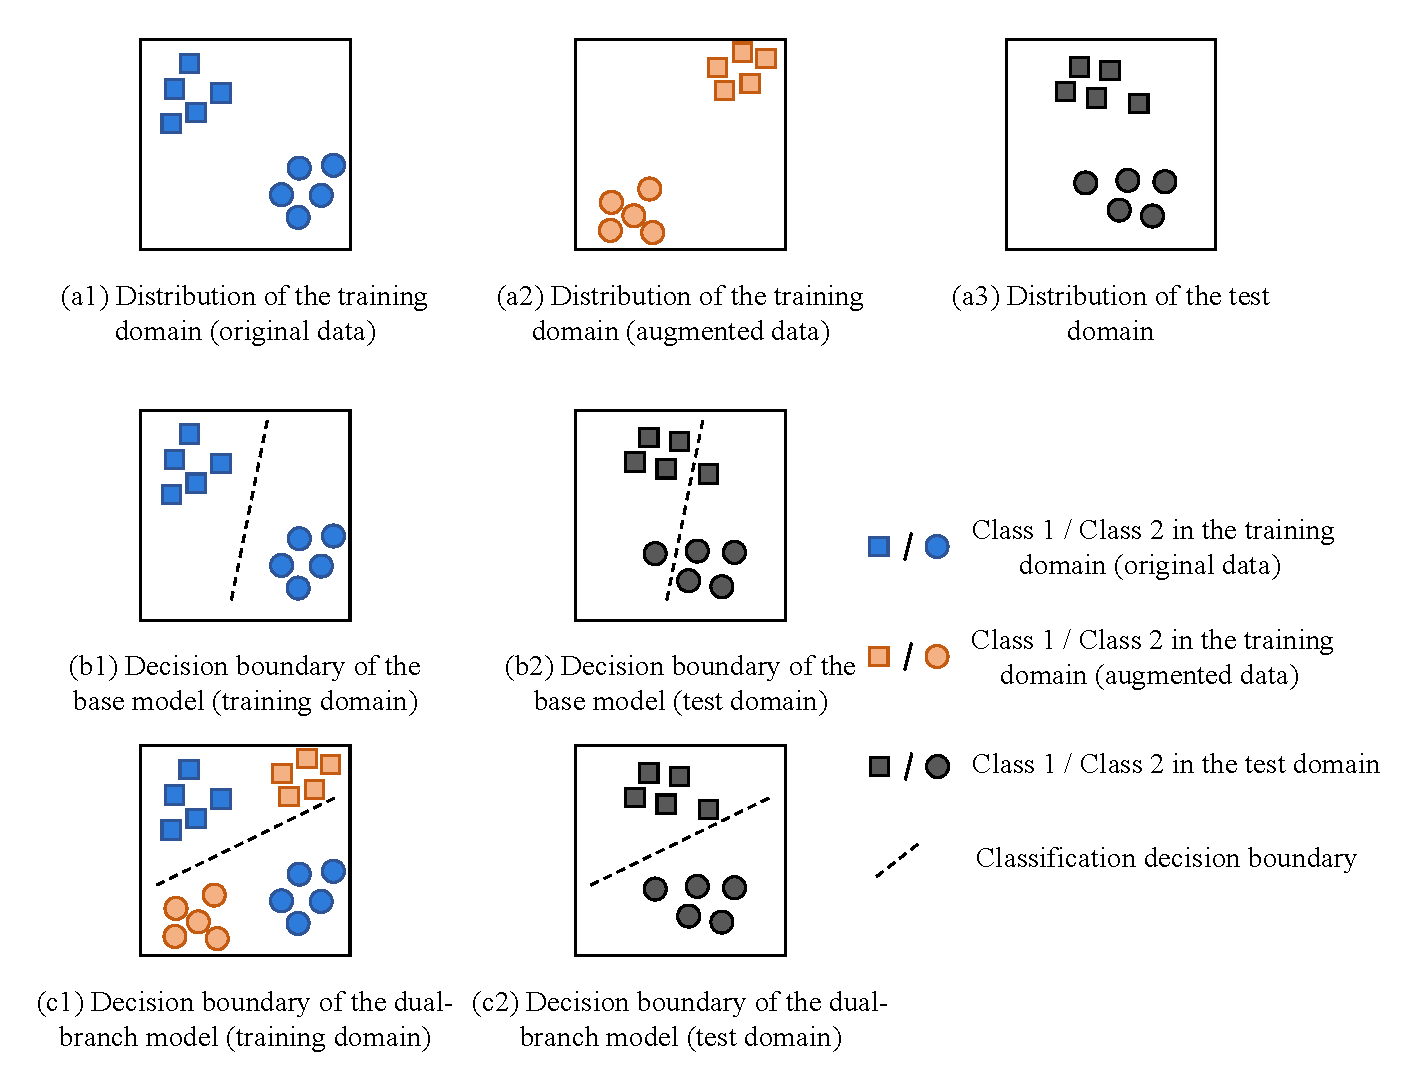
\includegraphics[width=0.72\textwidth]{images/media/image1_padded.pdf}
\caption{Schematic illustration of the decision boundaries of a conventional model and a dual-branch model under domain shift. (a) shows the distribution relationship among original source-domain images (training set), augmented source-domain images, and the target domain (test set), where augmented source-domain images are used to simulate possible distribution shifts in the target domain. (b) When the model is trained only with original source-domain images, the learned decision boundary may not fit the target domain and can therefore cause classification errors on target-domain samples. (c) By constructing a dual-branch structure with original and augmented source-domain images and incorporating contrastive learning with CAM guidance, the model extracts domain-invariant features and learns a decision boundary that is more applicable to unseen domains.}
\label{fig:intro-domain-gap}
\end{figure}

3. In fact, one of the key reasons behind the aforementioned restrictions on cross-institutional data sharing and multi-source collaborative training is precisely the privacy sensitivity of medical image data itself. Medical data are more sensitive than natural images and therefore involve higher privacy leakage risk. Common attack methods can recover patient data from model training gradients \cite{_Ref213949393}. To address this issue, privacy-preserving methods such as federated learning, homomorphic encryption, secure multi-party computation, and differential privacy have been investigated. However, privacy preservation usually comes with a privacy-performance trade-off. In DA scenarios in particular, source-domain and target-domain data must participate in training simultaneously, which can complicate the integration of privacy mechanisms and cause more severe performance degradation across domains. Therefore, a more reasonable approach is to explore the balance between privacy preservation and model performance within the local training process of a single source domain, without introducing cross-institutional data sharing.

To address the above three key challenges, we build a privacy-preserving interpretable single-domain generalization framework for multi-label ocular disease recognition. For the common issue of multi-disease co-occurrence in ocular disease recognition, we introduce a Transformer-based Adaptive Label-Feature Relevance Construction (ARC) module. It models label relevance using Transformer self-attention and fuses label semantics with corresponding image features using Transformer cross-attention, thereby constructing disease co-occurrence dependencies at both the label and feature levels to reduce false positives and false negatives in multi-label recognition. To handle restricted multi-institutional data access together with cross-institutional domain shift, we propose a Dual-Branch Guided Domain-Invariant Feature Extraction (DFE) module. This module is trained using only a single source domain and constructs a dual-branch structure from original source-domain images and style-disturbed augmented source-domain images, as shown in \hyperref[fig:intro-domain-gap]{Fig.~\ref*{fig:intro-domain-gap}.a1} and \hyperref[fig:intro-domain-gap]{Fig.~\ref*{fig:intro-domain-gap}.a2}, to learn their shared representations at the feature level. Meanwhile, Class Activation Mapping (CAM) is introduced as prior guidance to encourage the model to focus on disease-related regions and suppress the learning of domain-specific noise. This enables the model to form a decision boundary that is more suitable for unseen-domain distributions (\hyperref[fig:intro-domain-gap]{Fig.~\ref*{fig:intro-domain-gap}.c1}) and to maintain stable recognition performance on unseen domains (\hyperref[fig:intro-domain-gap]{Fig.~\ref*{fig:intro-domain-gap}.c2}). In addition, CAM visualizes model-attended regions and enhances model interpretability. To address the privacy-preservation demand that becomes more prominent when cross-institutional data sharing is restricted, we integrate an Adaptive Gaussian Differential Privacy (AdaGDP) mechanism into the single-domain generalization training process and provide privacy preservation by injecting noise during gradient updates. Under a moderate privacy budget, this mechanism provides effective privacy preservation at a controllable performance cost, and the resulting private model still attains performance comparable to or even slightly better than the public official baseline, thereby jointly supporting cross-domain generalization and privacy preservation.

Finally, generalization experiments on several representative fundus image datasets show that the framework improves cross-domain multi-label recognition performance while maintaining good interpretability, and it remains stable under privacy-preserving scenarios.

The main contributions of this study are summarized as follows:

\begin{enumerate}
\item We propose an Adaptive Label-Feature Relevance Construction (ARC) module. Based on Transformer self-attention and cross-attention mechanisms, ARC models disease co-occurrence dependencies at both the label and feature levels, effectively reducing false positives and false negatives in multi-label ocular disease recognition.

\item We design a Dual-Branch Guided Domain-Invariant Feature Extraction (DFE) module. For scenarios where joint training with multi-institutional data is restricted and cross-institutional deployment involves domain shift, this module learns domain-invariant features from a single source domain through joint guidance from style disturbance and CAM. It improves generalization performance on unseen domains and enhances the interpretability of model predictions.

\item We integrate an Adaptive Gaussian Differential Privacy (AdaGDP) mechanism into the single-domain generalization training process. Without introducing target-domain data, the proposed mechanism achieves an effective balance between privacy preservation and cross-domain generalization performance, and shows that model performance can remain close to the public official baseline under moderate privacy preservation.
\end{enumerate}

The remainder of this paper is organized as follows. Section 2 reviews recent related work. Section 3 presents the proposed method in detail, and Section 4 reports the complete experimental settings and results. Section 5 concludes the paper and discusses future work.


\section{Related Work}

\subsection{Multi-Label Image Recognition}

Unlike single-label recognition, multi-label image recognition allows one image to be assigned to multiple non-mutually exclusive categories, and therefore requires careful handling of label co-occurrence, label relevance, and class imbalance \cite{_Ref213949872}. Early methods such as Binary Relevance \cite{_Ref213949896} usually decompose a multi-label task into multiple independent binary classification problems. Such methods tend to ignore label relevance and may lead to incomplete or inconsistent predictions in complex visual scenarios.

To alleviate these problems, recent multi-label image recognition methods have increasingly focused on label relevance modeling and sample imbalance. ML-GCN \cite{_Ref213949382} constructs a label graph from label co-occurrence statistics and propagates label relevance information through graph convolutional networks. Asymmetric Loss (ASL) \cite{_Ref213949927} introduces different focusing parameters for positive and negative samples and suppresses the loss contribution of easy negative samples through negative probability shifting, thereby alleviating positive-negative sample imbalance in multi-label recognition. Query2Label \cite{_Ref213950246} further uses a Transformer query mechanism to model label interactions and achieves strong performance on natural image datasets such as VOC \cite{_Ref213950282}. These studies show that explicitly or implicitly incorporating label relevance into the model can improve the completeness and accuracy of multi-label prediction.

In medical fundus images, multi-label recognition is clinically important because multiple diseases may occur simultaneously in the same eye, and ignoring disease co-occurrence relationships may cause false positives and false negatives \cite{_Ref213949362}. Existing studies have explored multi-label ocular disease recognition from different perspectives. For example, Cheng et al. \cite{_Ref213950349} transferred ML-GCN to multi-label recognition of fundus lesions and modeled lesion label relevance by constructing a fundus lesion corpus and GloVe label representations. DCNet, proposed by He et al. \cite{_Ref213950338}, captures pixel-level relevance between left-eye and right-eye fundus image features through a spatial correlation module and fuses binocular features for patient-level multi-label ocular disease recognition. DKCNet \cite{_Ref213950343} uses an attention module to generate discriminative regional features and combines channel recalibration with resampling strategies to alleviate class imbalance in ocular datasets.

Overall, existing methods have partially addressed label relevance modeling and class imbalance. However, in fundus images with multi-disease co-occurrence, disease relationships are complex and lesion manifestations are often localized. Relying only on disease co-occurrence statistics or generic attention mechanisms may still be insufficient to characterize label-feature relevance reliably. Therefore, adaptive label-feature relevance construction for fundus images remains an important research problem. Building on label relevance modeling, this study couples adaptive label-feature relevance construction with single-source domain-invariant feature learning to address disease co-occurrence and cross-dataset application needs.

\subsection{Domain Generalization}

In computer vision tasks, a model may perform well on training data but degrade when deployed on data collected by new institutions or devices because of differences in imaging conditions, illumination environments, and data distributions. This domain shift is especially prominent in medical imaging, where differences among hospitals, devices, and acquisition procedures can directly affect model generalization \cite{_Ref213949439}. Domain Adaptation (DA) is a common approach for alleviating domain shift, with the core idea of aligning distributions using both source-domain and target-domain data during training. For example, maximum-mean-discrepancy-based Deep Domain Confusion \cite{_Ref213949448} and the correlation alignment method CORAL \cite{_Ref213949453} improve transfer performance by reducing feature distribution differences. DANN \cite{_Ref213949479} uses adversarial training to learn domain-invariant features. CycleGAN \cite{_Ref213949490} and related unsupervised domain adaptation methods \cite{_Ref213949530} alleviate domain shift through image style transfer or cross-domain contrastive learning. However, DA usually requires access to target-domain data during training, an assumption that often fails when medical data are privacy-sensitive or data from the target institution cannot be obtained in advance.

Unlike DA, Domain Generalization (DG) aims to learn domain-invariant features without accessing target-domain data and to generalize to unseen domains \cite{_Ref213949554}. Typical DG methods include MixStyle \cite{_Ref213949562}, which simulates potential domain shift by mixing instance style statistics; DomainBed \cite{_Ref213949607}, which provides a unified benchmark for evaluating DG algorithms; FACT \cite{_Ref213949788}, which decomposes domain-specific and domain-invariant information from a frequency-domain perspective; RSC \cite{_Ref213949796}, which suppresses dominant features to force the model to attend to more class-relevant cues; and meta-learning-based DG methods \cite{_Ref213949803}, which improve generalization by simulating differences between source and target domains. Most DG studies use multiple labeled source domains to learn cross-domain stable representations. This helps models capture richer inter-domain variations, but also requires consistent label spaces, coordinated data processing, and cross-institutional collaboration. In real-world medical scenarios, however, these conditions are not always available, making it difficult to centralize or synchronously use multi-institutional data. Even when centralized storage is avoided through federated learning, additional complexity arises from communication, privacy mechanisms, non-independent and identically distributed data, and collaborative optimization.

Against this background, Single-Domain Generalization (SDG) is a more constrained generalization setting that uses only one source domain to learn domain-invariant features for unseen domains. Studies on single-source DG in medical images \cite{_Ref213949863} also indicate that mining more stable disease-related features from a single source domain has practical value when multi-institutional data cannot be centrally used. In summary, the assumptions of target-domain accessibility or multi-source collaboration presumed by common cross-domain methods are difficult to satisfy simultaneously in real-world medical scenarios. Therefore, learning domain-invariant features from a single source domain is well aligned with the deployment constraints of cross-institutional multi-label ocular disease recognition.

\subsection{Privacy Preservation}

Medical images and electronic health records contain highly sensitive personal information, and model training, parameter sharing, or cloud inference may all introduce privacy leakage risk \cite{_Ref213950358}. In medical artificial intelligence applications, privacy preservation is tied not only to patient rights but also to data compliance requirements. Common privacy-preserving approaches include federated learning, encrypted computation, secure multi-party computation, and differential privacy. Among them, Federated Learning (FL) allows multiple clients to train models locally and upload parameters or gradients, thereby reducing the need for centralized sharing of raw data \cite{_Ref213950376}. For example, FedProx \cite{_Ref213950391} handles heterogeneous client data by adding a proximal term, alleviating instability in collaborative optimization.

Beyond federated learning, encryption mechanisms can provide stronger privacy preservation against privacy leakage. Homomorphic Encryption (HE) allows computation over ciphertexts \cite{_Ref213950427} and has been explored for medical image analysis \cite{_Ref213950433}, but it usually incurs high computational overhead. Secure Multi-Party Computation (SMPC) \cite{_Ref213950438} can protect the input privacy of each party during multi-party collaboration. Differential Privacy (DP) injects noise into query results or training gradients to provide quantifiable constraints on the privacy leakage risk of individual samples \cite{_Ref213950443}. Among DP mechanisms, Gaussian differential privacy \cite{_Ref213950449} injects Gaussian noise into clipped gradients and provides quantifiable privacy preservation for continuous gradient updates, making it well suited to gradient protection in deep learning.

Existing privacy-preserving mechanisms can reduce privacy leakage risk, but they still face additional challenges in domain generalization tasks. Federated learning, homomorphic encryption, and secure multi-party computation often introduce communication, computation, or system-level collaboration costs. Differential privacy is relatively straightforward to deploy, but noise injection may affect model accuracy, and this effect may vary across classes or data distributions \cite{_Ref213950458}. These issues make privacy preservation more challenging under multi-domain generalization. In summary, the privacy sensitivity of medical data further restricts cross-institutional data sharing and makes the aforementioned multi-source collaboration assumption even harder to hold. Therefore, controlling the privacy-performance trade-off during local single-source training is important for cross-institutional multi-label ocular disease recognition. Building on Gaussian gradient perturbation, this study adjusts noise intensity over training to examine this trade-off within the proposed framework.


\section{Proposed Method}

In domain generalization for multi-label ocular disease recognition, model performance is mainly affected by three factors. First, multiple diseases may coexist in the same fundus image. If the model cannot effectively capture relevance among disease labels and between labels and disease-related features, false positives and false negatives may occur, degrading multi-label recognition performance. Second, distribution shifts commonly arise between the source domain and target domain. If the learned features contain substantial source-domain-specific noise, the transferability of disease-related features is weakened, resulting in poorer domain generalization performance. In addition, medical data are privacy-sensitive, and the gradients or parameters produced during training may introduce privacy leakage risk, requiring a privacy-preserving mechanism to be incorporated into the training process. However, privacy-preserving mechanisms usually affect model optimization through additional training constraints, so the balance between privacy preservation and model performance must be considered.

To address these issues, this study does not treat multi-disease co-occurrence and domain shift as separate problems. Instead, they are jointly modeled within a single-domain generalization framework for multi-label ocular disease recognition. As shown in \hyperref[fig:method-framework]{Fig.~\ref*{fig:method-framework}}, the proposed interpretable single-domain generalization framework consists of two main parts: Part 1, Dual-Branch Guided Domain-Invariant Feature Extraction (DFE), and Part 2, Adaptive Label-Feature Relevance Construction (ARC). Part 1 uses CAM guidance together with a dual-branch mask-based contrastive learning mechanism to extract more stable domain-invariant features from a single source domain, thereby reducing the influence of distribution shift between the source domain and unseen domains. CAM also visualizes model-attended regions and enhances interpretability. Based on the domain-invariant features produced by Part 1, Part 2 uses Transformer attention mechanisms to model label-label relevance and label-feature relevance, reducing false positives and false negatives in multi-label recognition. These two parts are coupled through feature filtering and attention consistency constraints: Part 1 provides more stable domain-invariant features for Part 2, while Part 2 further constrains the consistency of dual-branch attention features, jointly improving domain generalization performance. Finally, an Adaptive Gaussian Differential Privacy mechanism is integrated during training to reduce the impact of privacy preservation on model performance and to balance privacy preservation with model performance. Overall, the proposed method constructs a Privacy-Preserving Interpretable Single-Domain Generalization framework for multi-label ocular disease recognition. The implementation details of each module are described in the following three subsections.

\begin{figure}
\centering
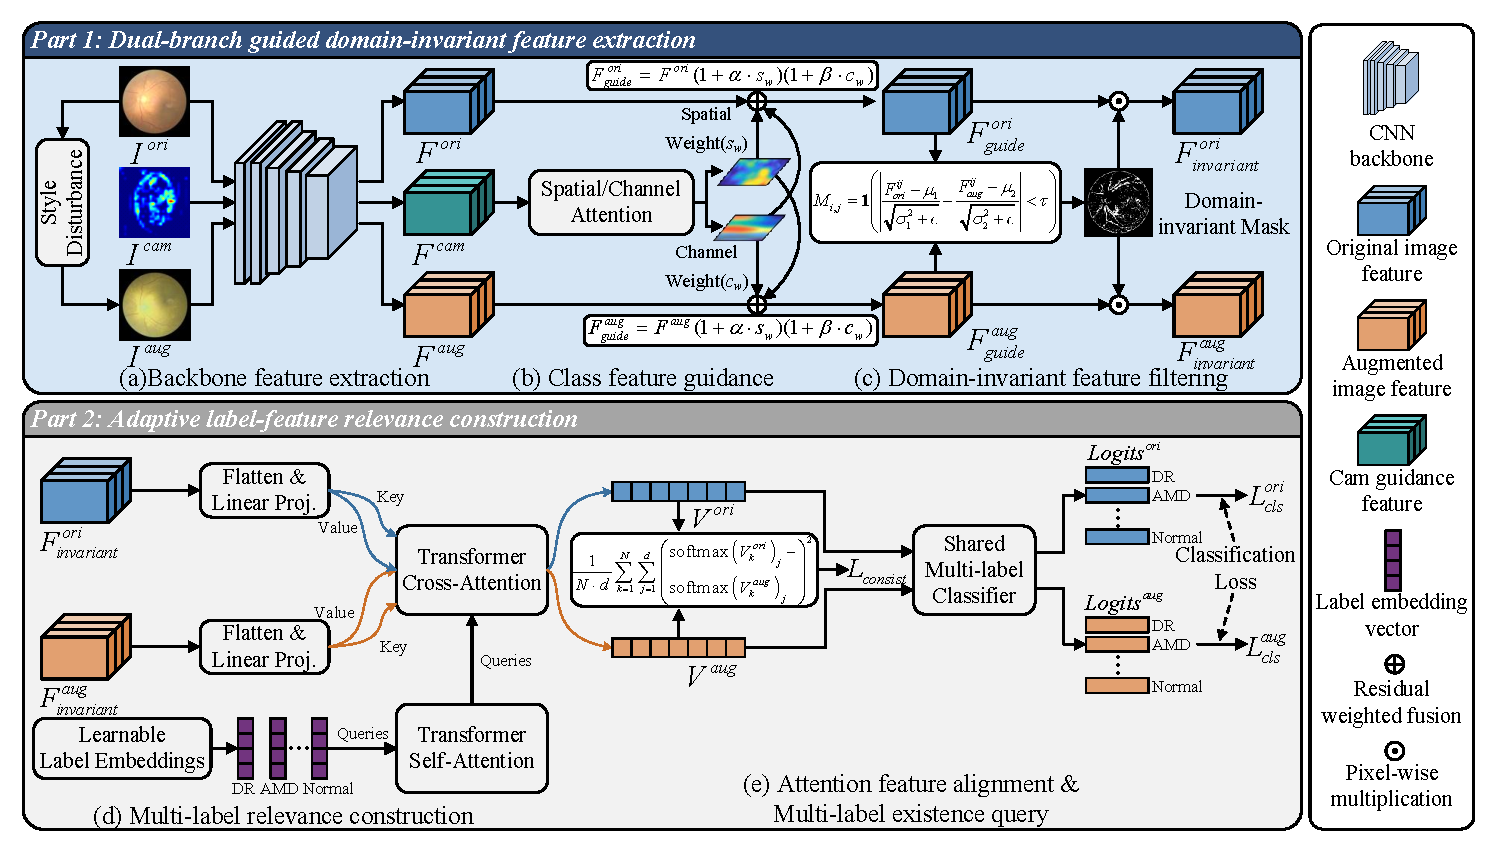
\includegraphics[width=0.96\textwidth]{images/media/image2_padded.pdf}
\caption{Overview of the proposed interpretable single-domain generalization framework. Part 1 is Dual-Branch Guided Domain-Invariant Feature Extraction (DFE), consisting of (a)--(c): (a) original source-domain images and augmented source-domain images are first fed into the backbone to extract dual-branch features; (b) CAM is used to generate model-attended region guidance, which enhances disease-related regions and suppresses background noise; and (c) a dual-branch mask-based contrastive learning mechanism retains highly similar components between the two feature branches to extract domain-invariant features. Part 2 is Adaptive Label-Feature Relevance Construction (ARC), consisting of (d)--(e): (d) Transformer self-attention is used to model label-label relevance, and cross-attention is then used to establish label-feature relevance; (e) attention consistency constraints improve the stability of attention features, thereby reducing false positives and false negatives in multi-label recognition.}
\label{fig:method-framework}
\end{figure}

\subsection{Dual-Branch Guided Domain-Invariant Feature Extraction}

Considering that multi-institutional data in medical scenarios are often difficult to centralize or use synchronously, this study adopts a single-domain generalization setting and learns domain-invariant features for unseen-domain data using only one source domain. Inspired by contrastive learning, original source-domain images are transformed into augmented source-domain images through augmentation techniques such as style disturbance to simulate possible distribution shifts in unseen domains. Specifically, \(I^{ori}\) denotes original source-domain images, and \(I^{aug}\) denotes augmented source-domain images generated by style disturbance, such as MixStyle or random adjustment of brightness, contrast, and saturation. This augmentation simulates differences in imaging devices, illumination environments, or patient populations in cross-domain scenarios while preserving the semantic content of the images, namely disease regions.

First, as shown in \hyperref[fig:method-framework]{Fig.~\ref*{fig:method-framework}.a}, both \(I^{ori}\) and \(I^{aug}\) are fed into the backbone network to extract features \(F^{ori}\) and \(F^{aug}\). Let \(F^{ori} \in \mathbb{R}^{C \times H \times W}\) and \(F^{aug} \in \mathbb{R}^{C \times H \times W}\), where \(C\), \(H\), and \(W\) denote the number of channels, height, and width of the final feature map of the backbone network, respectively. ResNet50 \cite{_RefResNet2016} is selected as the backbone because it performs well in image recognition tasks and offers good feature extraction capability and computational efficiency. However, relying only on contrastive constraints between original and augmented source-domain images remains limited. The model may still learn domain-specific noise such as background textures, illumination variations, or image-edge artifacts, which can affect multi-label ocular disease recognition on unseen domains.

To this end, we introduce the class feature guidance module shown in \hyperref[fig:method-framework]{Fig.~\ref*{fig:method-framework}.b} to improve the disease relevance and interpretability of features. A CAM guidance map is generated on the training set in advance using the baseline model, namely ResNet50 with BCE loss. The CAM guidance map highlights the regions attended by the model for different diseases; for example, Diabetic Retinopathy (DR) mainly corresponds to vascular regions, whereas Age-Related Macular Degeneration (AMD) mainly corresponds to the macular region. For a target class \(c\), it is calculated as follows:

\begin{equation}\label{eq:cam}
I^{cam,c} = \operatorname{ReLU}\left(\sum_{k = 1}^{C}\omega_{k}^{c} \cdot A_{k}\right),
\end{equation}

Here, \(A_{k}\) is the activation map of the \(k\)-th channel in the last convolutional layer of the backbone network, and \(\omega_{k}^{c}\) is the importance weight of the \(k\)-th channel for target class \(c\). It is obtained by global average pooling the gradient of the class score \(y^{c}\) with respect to the channel activation map:

\begin{equation}\label{eq:cam-weight}
\omega_{k}^{c} = \frac{1}{Z}\sum_i\sum_j \frac{\partial y^{c}}{\partial A_{ij}^{k}},
\end{equation}

where \(Z\) denotes the number of spatial locations in the feature map. This Grad-CAM-based formula produces a class-specific spatial attention heatmap rather than a raw fundus image. In practice, one or more \(I^{cam,c}\) maps are generated according to the positive labels or predicted classes of an image, and they are normalized and resized to form the CAM guidance map \(I^{cam}\). The resulting \(I^{cam}\) is then fed into the backbone network to obtain \(F^{cam} \in \mathbb{R}^{C \times H \times W}\). Spatial attention weights \(s_{w}\) and channel attention weights \(c_{w}\) are then computed from \(F^{cam}\) through spatial and channel attention modules, respectively. Both attention modules are convolutional sequential networks containing \(1 \times 1\) convolution, ReLU activation, and a Sigmoid function for adaptive weight generation. The spatial attention module additionally combines average and max pooling to capture local context, generating a pixel-level weight map that adaptively enhances the saliency of lesion regions, such as vessels or the macula, while suppressing background noise. The channel attention module uses adaptive average pooling to compress spatial dimensions and obtain global statistics, then learns channel dependencies to enhance disease-texture-sensitive channels and suppress noisy channels. The two weights are applied to \(F^{ori}\) and \(F^{aug}\) to obtain CAM-guided features \(F_{guide}^{ori}\) and \(F_{guide}^{aug}\). A residual connection is used in the weighting operation to avoid damaging original information through excessive guidance:

\begin{align}
F_{guide}^{ori} &= F^{ori}(1 + \alpha{\cdot s}_{w})(1 + {\beta \cdot c}_{w}), \label{eq:guide-feature-ori} \\
F_{guide}^{aug} &= F^{aug}(1 + \alpha{\cdot s}_{w})(1 + {\beta \cdot c}_{w}), \label{eq:guide-feature-aug}
\end{align}

Here, \(\alpha\) and \(\beta\) are hyperparameters that control the enhancement strengths of \(s_{w}\) and \(c_{w}\), respectively. Residual weighting allows CAM guidance to highlight disease-related regions while retaining the original feature representation, reducing the model's reliance on domain-specific noise such as illumination and background textures. Extracting domain-invariant features from these guided representations helps improve the disease relevance of the learned features. Meanwhile, visualizing model-attended regions through CAM enhances model interpretability and helps clinicians understand the basis of prediction, for example by overlaying CAM to inspect whether the model focuses on lesion regions.

Next, we introduce the domain-invariant feature filtering module, as shown in \hyperref[fig:method-framework]{Fig.~\ref*{fig:method-framework}.c}. This study adopts a dual-branch mask-based contrastive learning mechanism to compute the similarity between guided features from original source-domain images and augmented source-domain images at the feature-distribution level. Highly similar components represent disease-related regions that remain stable under style disturbance and are therefore retained, whereas low-similarity components are more likely to contain domain-specific noise caused by illumination, device style, or style disturbance and are therefore suppressed. The mask matrix \(M \in \mathbb{R}^{C \times H \times W}\) is calculated from the normalized distance:

\begin{equation}\label{eq:mask}
M_{ij} =
\left\{
\begin{array}{ll}
1, & \text{if } \left| \dfrac{F_{guide}^{ori,ij} - \mu_{1}}{\sqrt{\sigma_{1}^{2} + \epsilon}} - \dfrac{F_{guide}^{aug,ij} - \mu_{2}}{\sqrt{\sigma_{2}^{2} + \epsilon}} \right| \leq \tau, \\
0, & \text{otherwise.}
\end{array}
\right.
\end{equation}

Here, \(\mu_{1},\sigma_{1}\) and \(\mu_{2},\sigma_{2}\) are the means and variances of the two guided features, respectively, \(\epsilon = 10^{-5}\) is a stability constant, and \(i,j\) denote feature map positions. Components satisfying the threshold \(\tau\) are assigned 1, while the remaining components are assigned 0. The mask matrix is then applied to \(F_{guide}^{ori}\) and \(F_{guide}^{aug}\) to extract domain-invariant features:

\begin{equation}\label{eq:invariant-feature}
F_{invariant}^{ori} = F_{guide}^{ori} \odot M,F_{invariant}^{aug} = F_{guide}^{aug} \odot M,
\end{equation}

Here, \(\odot\) denotes pixel-wise element-wise multiplication, ensuring that only shared disease-related features, such as vascular or macular textures, are retained while illumination or device noise is removed. The resulting \(F_{invariant}^{ori}\) and \(F_{invariant}^{aug}\) are used as inputs for subsequent label-feature relevance construction, enabling multi-label relevance learning to be built on more stable domain-invariant features.

\subsection{Adaptive Label-Feature Relevance Construction}

After obtaining domain-invariant disease features, the model further handles the multi-label relevance problem caused by ocular disease co-occurrence. To this end, Transformer attention mechanisms are embedded to construct adaptive relevance at the label and feature levels for multi-label prediction. As shown in \hyperref[fig:method-framework]{Fig.~\ref*{fig:method-framework}.d} and \hyperref[fig:method-framework]{Fig.~\ref*{fig:method-framework}.e}, this module includes multi-label relevance construction and attention feature alignment.

First, the eight labels in the ODIR dataset, such as normal, DR, and AMD, are modeled as learnable vectors \(L = \lbrack L_{1},\ldots,L_{8}\rbrack \in \mathbb{R}^{8 \times d}\), where \(d = 512\) is the embedding dimension. These vectors are initialized from a random Gaussian distribution and optimized during training to characterize potential relevance among different disease labels. The label vectors are fed into the Transformer self-attention mechanism to model label relevance:

\begin{equation}\label{eq:self-attention}
V_{self} = \operatorname{softmax}\left(\frac{QK^{T}}{\sqrt{d_{k}}}\right)V,
\end{equation}

Here, \(Q = LW_{Q},K = LW_{K},V = LW_{V}\), where \(W_{Q},W_{K},W_{V}\) are learnable projection matrices and \(d_{k} = d/heads\) for multi-head attention with \(heads=8\). The self-attention output \(V_{self}\) captures label relevance, enabling different disease labels to interact dynamically according to co-occurrence patterns and visual evidence in the training data.

Next, a cross-attention mechanism is used to combine labels with domain-invariant features. Since Transformer requires sequential input, \(F_{invariant}^{ori}\) and \(F_{invariant}^{aug}\) output by Part 1 are first flattened and used as Key and Value, while the label vector \(V_{self}\) is used as Query for cross-attention calculation:

\begin{equation}\label{eq:cross-attention}
V_{cross}^{ori} = \operatorname{softmax}\left(\frac{V_{self}W_{Q}(F_{invariant}^{ori}W_{K})^{T}}{\sqrt{d_{k}}}\right)(F_{invariant}^{ori}W_{V}),
\end{equation}

\(V_{cross}^{aug}\) is calculated in the same way. Through cross-attention weighting, labels are matched with corresponding disease features to form attention vectors \(V \in \mathbb{R}^{8 \times d}\), so that each label vector obtains a higher response on disease-related regions. In this process, each label vector is not matched with image features independently; instead, it queries image features based on the label relevance modeled by self-attention. The model can therefore focus on local lesion features corresponding to each disease while also using disease co-occurrence dependencies to support the prediction of other relevant labels, thereby reducing false positives and false negatives in multi-label recognition.

To ensure consistency between the outputs of the two branches, we introduce an attention consistency constraint and compute an attention consistency loss. Original source-domain images and augmented source-domain images share the same disease labels and differ only in style. Therefore, the corresponding label attention vectors should remain close. This loss encourages consistent attention features across the two branches, enabling the model to learn similar label-feature relevance from inputs with different styles. It is calculated using mean squared error (MSE):

\begin{equation}\label{eq:consistency-loss}
L_{consist} = \frac{1}{N \cdot d}\sum_{k = 1}^{N}\sum_{j = 1}^{d}
\left(
\operatorname{softmax}\left( V_{k}^{ori} \right)_{j}
-
\operatorname{softmax}\left( V_{k}^{aug} \right)_{j}
\right)^{2},
\end{equation}

Here, \(N = 8\) is the number of labels and \(d = 512\) is the embedding dimension. Softmax normalizes attention vectors into comparable distribution forms. The attention consistency loss improves model stability under domain shift by minimizing differences between normalized attention features of the two branches.

Finally, the attention vectors are fed into the multi-label classifier. LayerNorm and Dropout are first applied to the class query features for lightweight feature enhancement, normalization, and regularization. Class-wise linear transformations are then used to obtain logits for each class. After Sigmoid activation, the prediction probabilities \(p^{ori}\) are obtained for each class, and \(p^{aug}\) is obtained in the same way. The classification loss uses binary cross entropy (BCE):

\begin{equation}\label{eq:cls-loss}
L_{cls}^{ori} = - \frac{1}{8}\sum_{k = 1}^{8}{\lbrack y_{k}\log p_{k}^{ori} + (1 - y_{k})\log(1 - p_{k}^{ori})\rbrack},
\end{equation}

The total loss is \(L = L_{cls}^{ori} + L_{cls}^{aug} + \lambda L_{consist}\), where \(\lambda\) is a hyperparameter that balances the consistency term. Through this design, the DFE module provides disease-related domain-invariant features for the ARC module, and the ARC module further models label-label relevance and label-feature relevance. The two modules work together to improve multi-label recognition capability in cross-domain scenarios.

\subsection{Integration of Privacy Preservation}

Medical image data are highly sensitive, and gradients or model parameters generated during training may leak sample information. In particular, gradient inversion attacks may even recover original images, leading to privacy leakage risk. To balance privacy preservation and model performance in single-domain generalization models, this study introduces an Adaptive Gaussian Differential Privacy (AdaGDP) mechanism. The overall privacy-preserving framework is shown in \hyperref[fig:privacy-framework]{Fig.~\ref*{fig:privacy-framework}}.

\begin{figure}
\centering
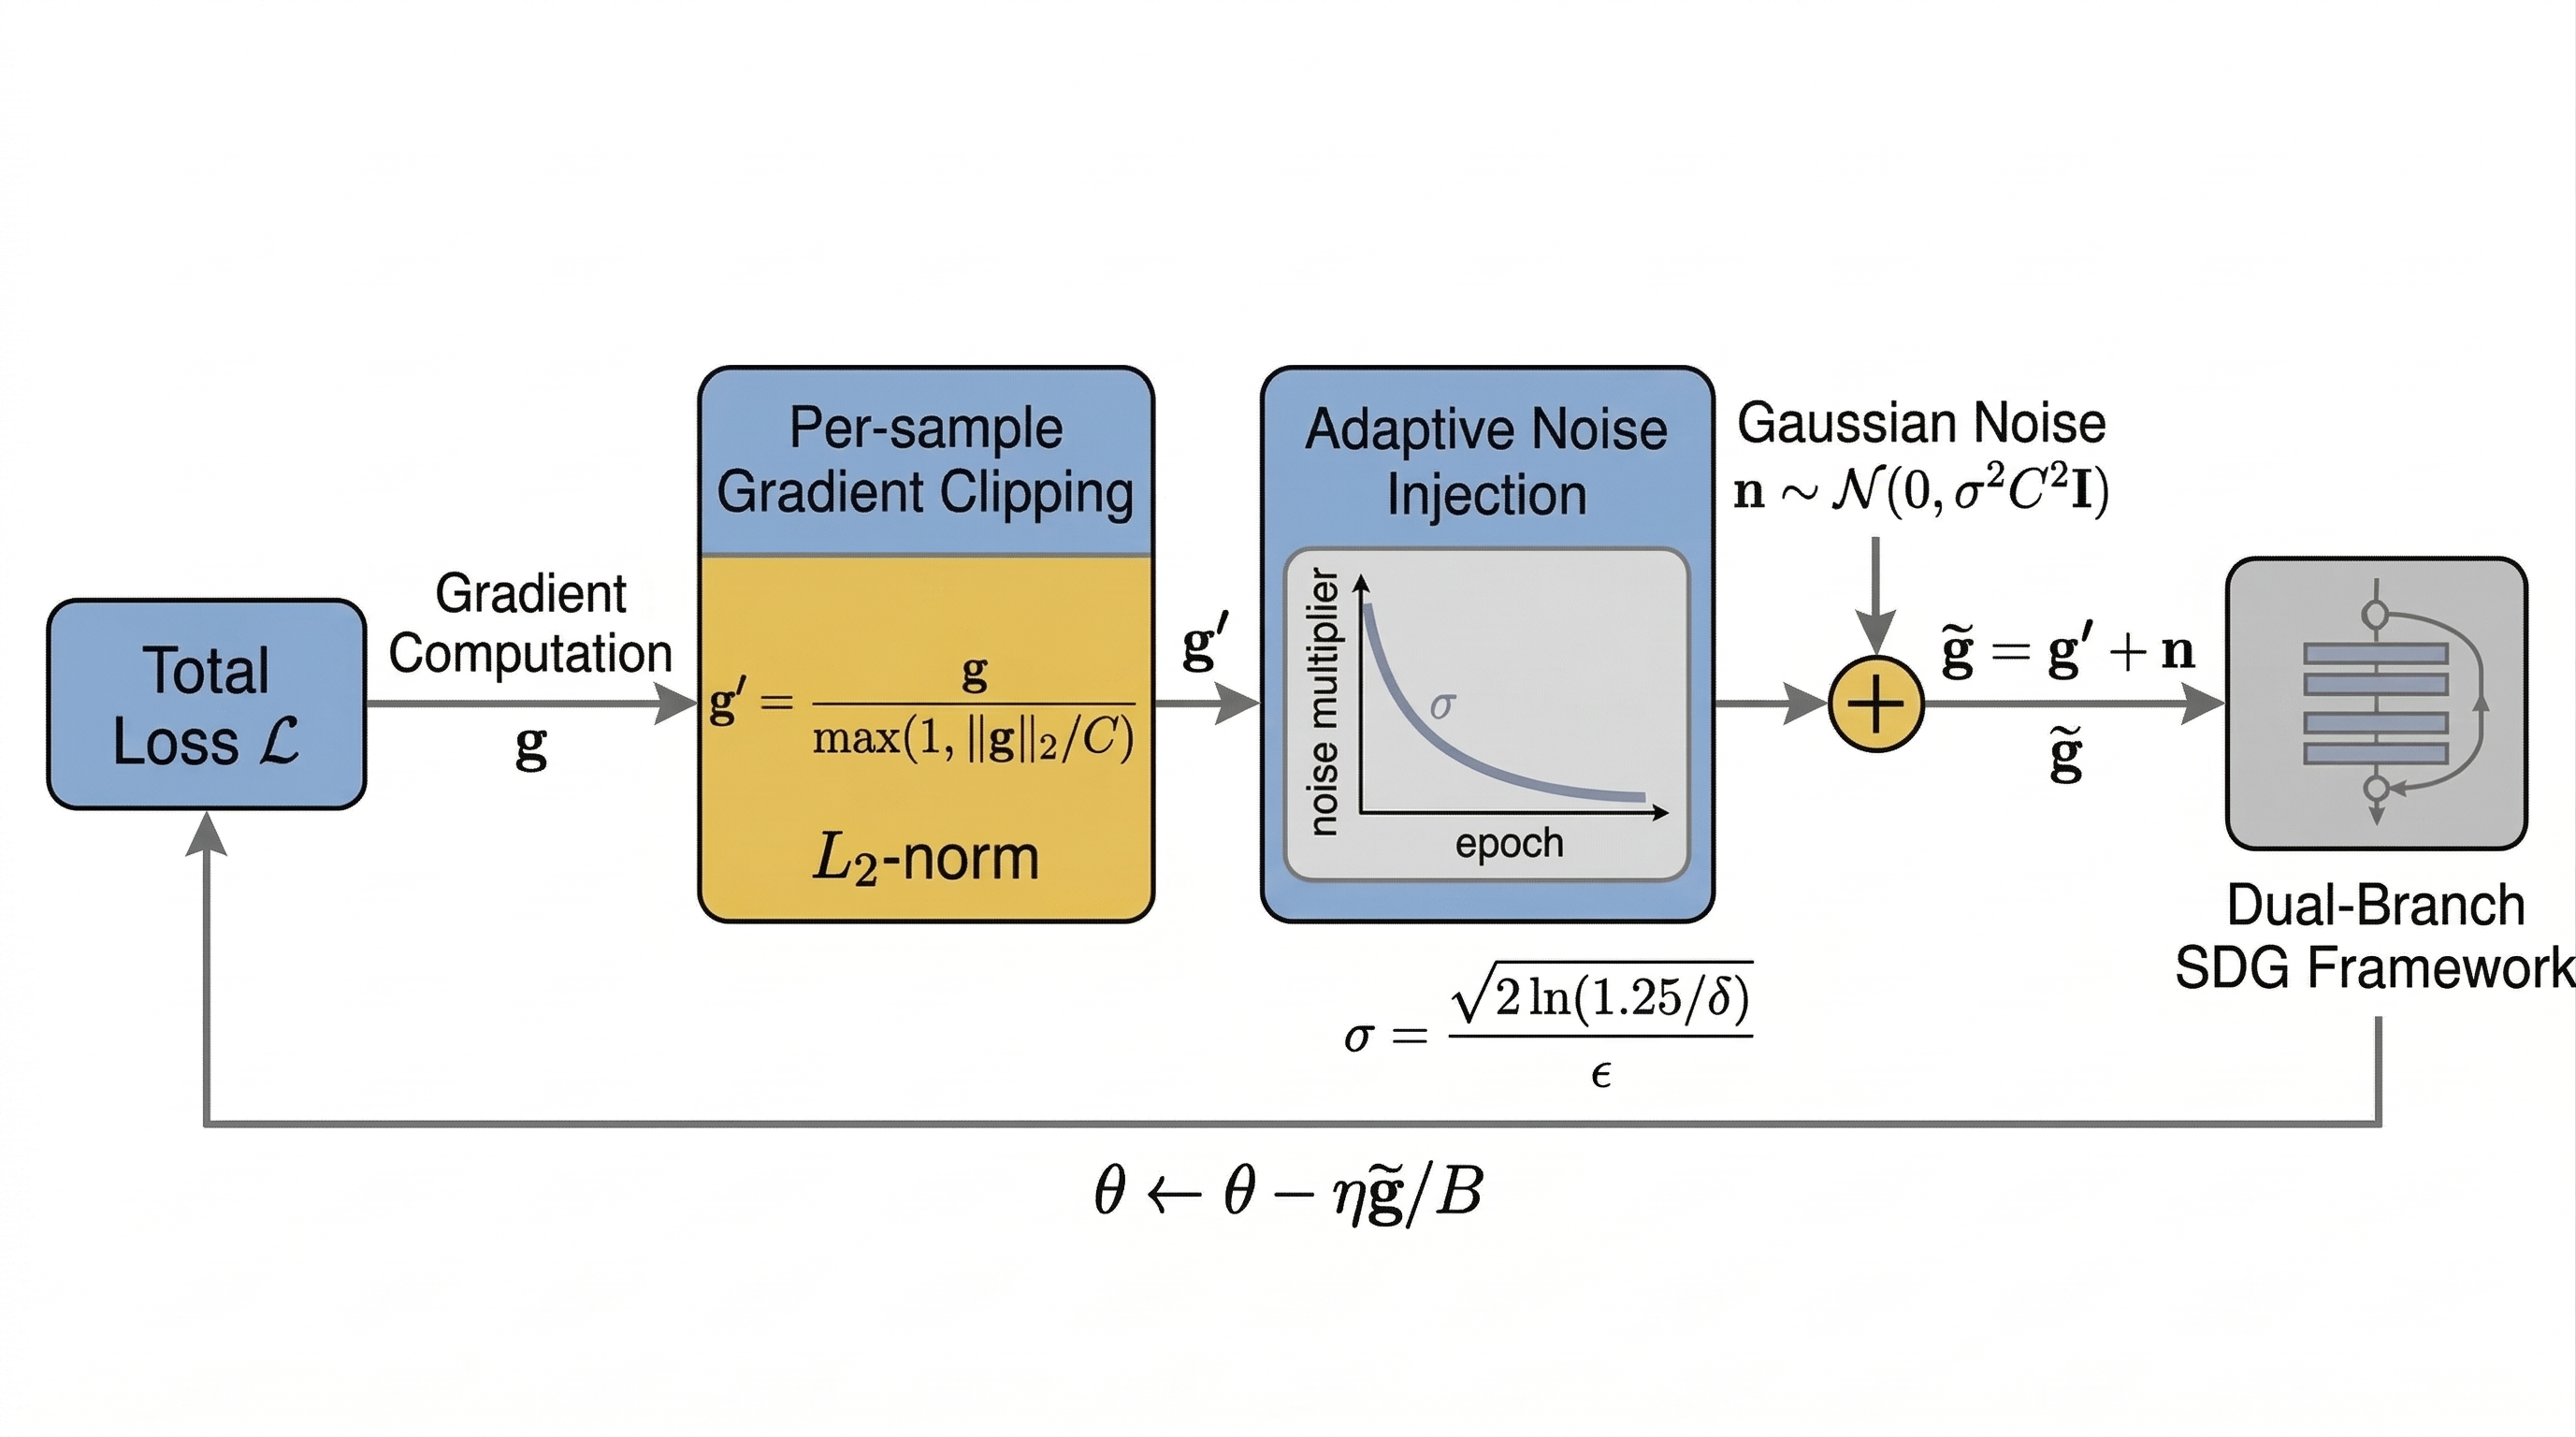
\includegraphics[width=0.82\textwidth]{images/media/image3_v2.png}
\caption{Integration of Adaptive Gaussian Differential Privacy into the single-domain generalization framework. During training, each update first clips per-sample gradients, then injects Gaussian noise and updates the parameters. Unlike fixed-noise differential privacy, this study adopts a noise multiplier that is adaptively adjusted and gradually decayed with the training stage.}
\label{fig:privacy-framework}
\end{figure}

Gaussian differential privacy (GDP) provides \((\epsilon, \delta)\)-differential privacy by adding independent and identically distributed Gaussian noise at each gradient update. For adjacent datasets \(D\) and \(D'\), which differ by only one sample, a randomized algorithm \(M\) satisfies \((\epsilon, \delta)\)-DP if, for any output set \(S\), it satisfies:

\begin{equation}\label{eq:dp-definition}
\Pr\lbrack M(D) \in S\rbrack \leq e^{\epsilon}\Pr\lbrack M(D') \in S\rbrack + \delta,
\end{equation}

where \(\epsilon\) measures the degree of privacy preservation, and \(\delta\) is the relaxation parameter, usually set to \(10^{-5}\). Under the DP-SGD framework, the per-sample gradient \(g\) is first clipped by its L2 norm at each iteration:

\begin{equation}\label{eq:gradient-clip}
g' = g/max(1, \parallel g \parallel_{2}/C),
\end{equation}

Gaussian noise \(n \sim \mathcal{N}(0,\sigma^{2}C^{2}I)\) is then added, where \(\sigma\) is the noise multiplier controlling noise intensity. It is usually related to the privacy budget \(\epsilon\) and relaxation parameter \(\delta\), and can be written as:

\begin{equation}\label{eq:noise-multiplier}
\sigma = \sqrt{2\ln(1.25/\delta)}/\epsilon.
\end{equation}

The noisy gradient is \(\widetilde{g} = g' + n\), and the parameters are updated as \(\theta \leftarrow \theta - \eta\widetilde{g}/B\), where \(B\) is the batch size. This process obscures gradients through noise injection and prevents inversion attacks from recovering original images or labels. Detailed theoretical guarantees for privacy-preserving mechanisms are provided by Dwork C et al. \cite{_Ref214903493}.

However, conventional GDP uses a fixed \(\sigma\) throughout training, so substantial noise is still injected in later training stages, which can affect model convergence and final performance. Therefore, we adopt an Adaptive Gaussian Differential Privacy optimizer. A larger noise multiplier is used early in training to provide stronger protection, and the noise intensity is then gradually reduced according to a predefined noise decay rate to limit the impact of noise on model convergence in later stages. During training, this study accumulates the privacy budget according to the noise multiplier, noise decay rate, and sampling process of each epoch, and records \(\epsilon\) consumption and model performance at different training epochs to analyze performance evolution as the privacy budget increases. The final experiments show that, under a moderate privacy budget, the proposed method can alleviate the performance degradation caused by noise injection and achieve a good balance between privacy preservation and model performance.


\section{Experiments}

\subsection{Datasets}

This study uses the ODIR-5K (Ocular Disease Intelligent Recognition) \cite{_Ref213949402} dataset as the single source domain. ODIR contains 10,000 color fundus images from 5,000 patients, with one left-eye and one right-eye image for each patient. The images were initially annotated by three ophthalmologists with more than two years of clinical experience and then adjudicated by three experts with more than ten years of experience. The dataset defines eight non-mutually exclusive classes: normal (N), Diabetic Retinopathy (D), Glaucoma (G), Cataract (C), Age-Related Macular Degeneration (A), Hypertension (H), Myopia (M), and Others (O), as shown in \hyperref[fig:odir-samples]{Fig.~\ref*{fig:odir-samples}.a} to \hyperref[fig:odir-samples]{Fig.~\ref*{fig:odir-samples}.h}. This setting is a typical multi-label ocular disease recognition task. Each image may have multiple disease labels, and patient-level labels are determined by combining diagnostic keywords from both eyes. The official split divides the 5,000 patients into three subsets: the training set with 3,500 patients for model training, the Off-site test set with 500 patients for model selection, and the On-site test set with 1,000 patients for evaluating in-domain generalization performance. The class distribution is shown in \hyperref[tab:dataset-distribution]{Table~\ref*{tab:dataset-distribution}}, indicating class imbalance.

% Chapter 4 Experiments - Table 1
% Label distribution across the ODIR training and test splits.
\begin{table}
\centering
\caption{Distribution of samples in each class of the ODIR dataset across the training set, On-site test set, and Off-site test set. The normal (N), Diabetic Retinopathy (D), and Others (O) classes contain relatively more samples, whereas Hypertension (H) has the fewest samples, indicating clear class imbalance.}
\label{tab:dataset-distribution}
\resizebox{\textwidth}{!}{
\begin{tabular}{lcccccccc}
\toprule
Labels & N & D & G & C & A & H & M & O \\
\midrule
Training & 1138 & 1130 & 215 & 212 & 164 & 103 & 174 & 982 \\
On-site test & 324 & 327 & 58 & 65 & 49 & 30 & 46 & 275 \\
Off-site test & 162 & 163 & 32 & 31 & 25 & 16 & 23 & 136 \\
All & 1624 & 1620 & 305 & 308 & 238 & 149 & 243 & 1393 \\
\bottomrule
\end{tabular}
}
\end{table}


\begin{figure}
\centering
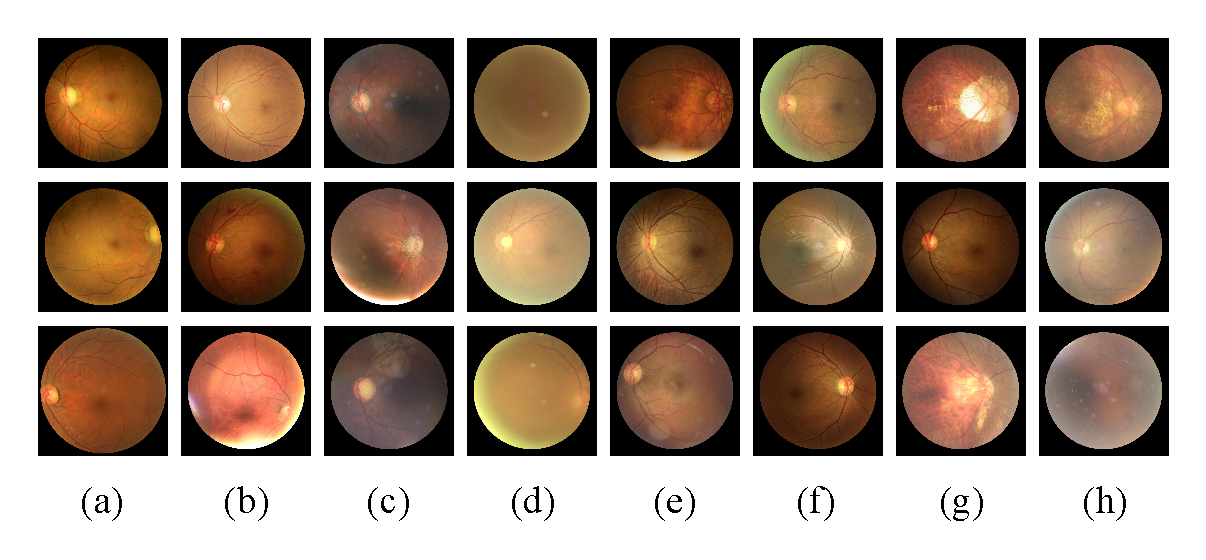
\includegraphics[width=0.86\textwidth]{images/media/image5_padded.pdf}
\caption{Example fundus images of the eight classes in the ODIR dataset, corresponding to the eight non-mutually exclusive classes used in this study. (a)--(h) denote (a) normal (N), (b) Diabetic Retinopathy (D), (c) Glaucoma (G), (d) Cataract (C), (e) Age-Related Macular Degeneration (A), (f) Hypertension (H), (g) Myopia (M), and (h) Others (O), respectively.}
\label{fig:odir-samples}
\end{figure}

To comprehensively evaluate domain generalization capability, in addition to ODIR in-domain generalization, this study introduces RFMiD \cite{_Ref213949409}, provided by the RIADD challenge, as the first independent cross-domain generalization dataset. RFMiD contains 3,200 color fundus images, with 1,920, 640, and 640 images in the training, validation, and test sets, respectively. It covers 45 retinal diseases or abnormalities annotated by professional retina specialists. Some of its 45 labels overlap with the eight labels in ODIR, providing a basis for model generalization. \hyperref[fig:rfmid-samples]{Fig.~\ref*{fig:rfmid-samples}.a} to \hyperref[fig:rfmid-samples]{Fig.~\ref*{fig:rfmid-samples}.h} show representative images from eight of the 45 categories. Since the complete label spaces of RFMiD and ODIR are inconsistent, this study selects their shared classes, Diabetic Retinopathy (D), Age-Related Macular Degeneration (A), and Myopia (M), for cross-domain generalization. Under this setting, 1,907 D/A/M training images are constructed on the ODIR side, with 1,425, 255, and 253 labels for D, A, and M, respectively. On the RFMiD side, 119 validation images from these three classes are used for testing, with 83, 24, and 21 labels for D, A, and M, respectively.

\begin{figure}
\centering
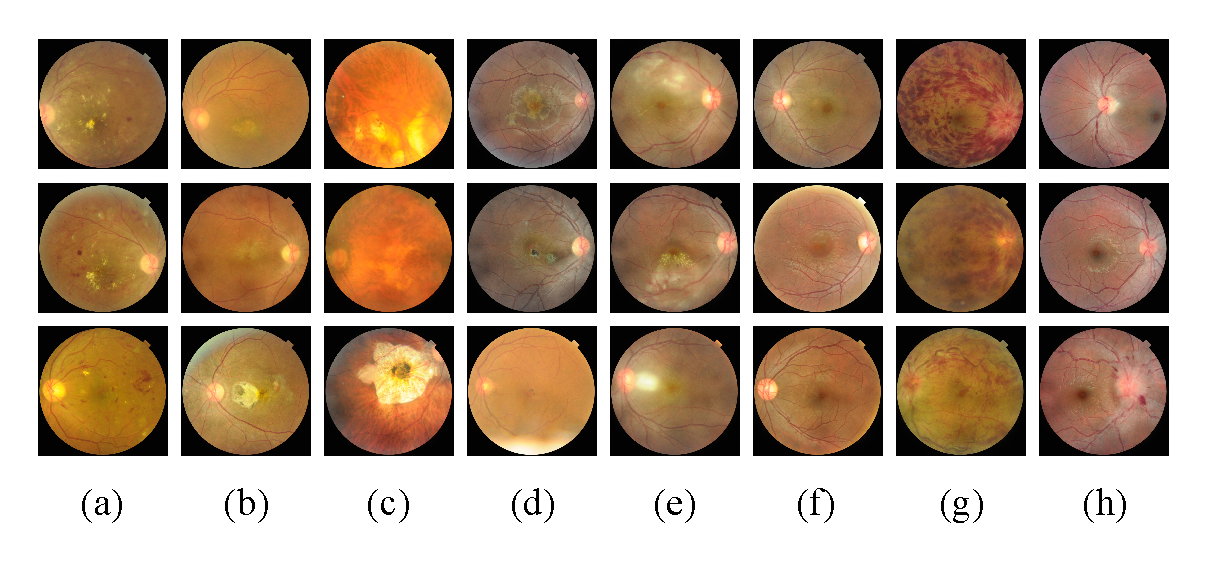
\includegraphics[width=0.86\textwidth]{images/media/image6_padded.pdf}
\caption{Examples of eight selected fundus image classes in the RFMiD dataset. (a)--(h) correspond to (a) Diabetic Retinopathy (D), (b) Age-Related Macular Degeneration (A), (c) Myopia (M), (d) Macular Scar (MS), (e) Retinitis (RS), (f) Central Serous Retinopathy (CSR), (g) Central Retinal Vein Occlusion (CRVO), and (h) Disc Edema (DE), respectively.}
\label{fig:rfmid-samples}
\end{figure}

In addition, this study introduces the EDID \cite{_RefEDID2024} dataset collected from Anawara Hamida and B.N.S.B. Zahurul Haque Eye Hospital as the second independent cross-domain generalization dataset, further validating the generalization performance of the proposed method across different data sources and label organizations. The original EDID dataset contains 5,335 fundus images covering 10 single-label classes, including Central Serous Retinopathy, Diabetic Retinopathy, Disc Edema, Glaucoma, normal, Macular Scar, Myopia, Pterygium, Retinal Detachment, and Retinitis Pigmentosa, with 101, 1,509, 127, 1,349, 1,024, 444, 500, 17, 125, and 139 samples, respectively. \hyperref[fig:edid-samples]{Fig.~\ref*{fig:edid-samples}.a} to \hyperref[fig:edid-samples]{Fig.~\ref*{fig:edid-samples}.h} show examples of eight representative fundus image classes selected from EDID.

\begin{figure}
\centering
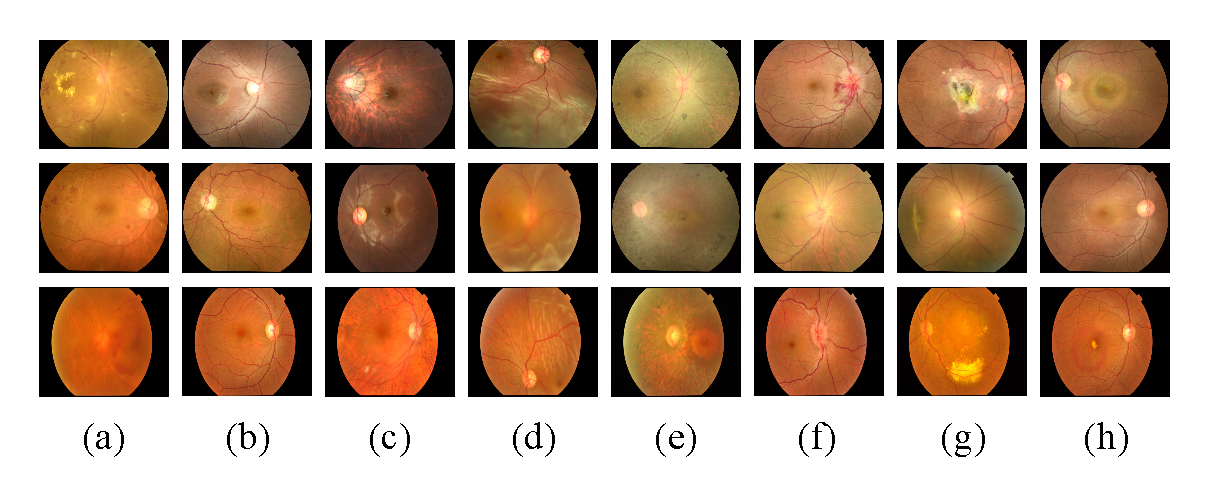
\includegraphics[width=0.86\textwidth]{images/media/edid_samples_padded.pdf}
\caption{Examples of eight selected fundus image classes in the EDID dataset. (a)--(h) correspond to (a) Diabetic Retinopathy (D), (b) Glaucoma (G), (c) Myopia (M), (d) Retinal Detachment (RD), (e) Retinitis Pigmentosa (RP), (f) Disc Edema (DE), (g) Macular Scar (MS), and (h) Central Serous Retinopathy (CSR), respectively.}
\label{fig:edid-samples}
\end{figure}

Similar to RFMiD, since the complete label spaces of EDID and ODIR are inconsistent, this study selects their shared classes, Diabetic Retinopathy (D), Glaucoma (G), and Myopia (M), to construct a cross-domain generalization dataset with 3,358 images, including 1,509, 1,349, and 500 samples for D, G, and M, respectively. Since EDID is a single-label dataset, it is treated as a special case of the multi-label recognition task, where each image has only one positive label, and cross-domain generalization is evaluated in the D/G/M three-class space. Correspondingly, a D/G/M training subset is constructed on the ODIR side, containing 1,871 images, with 1,401, 227, and 243 samples for D, G, and M, respectively.

\subsection{Experimental Settings}

All experiments use ResNet50 as the backbone and are implemented in PyTorch. The evaluation metrics follow the official ODIR standard: Kappa, F1, AUC, and their average value, Final score. The Kappa threshold is fixed at 0.5, and F1 uses micro averaging to alleviate the influence of class imbalance.

For the baseline, we follow the original ResNet50 implementation of ODIR and modify it for our setting. The original paper uses paired binocular samples as input, evaluates different feature-level fusion strategies such as concat, prod, and sum, and then uses eight independent classification heads for patient-level prediction. In contrast, we use monocular images as input samples, with each sample carrying its corresponding patient identifier. The classifier is implemented as a single multi-label classification head, which outputs eight-dimensional logits and obtains disease probabilities through Sigmoid activation. The loss function is standard binary cross entropy (BCE). During inference, monocular predictions from the left and right eyes of the same patient are logically merged to obtain patient-level predictions, fully aligning with the official metrics. This modification avoids noise amplification caused by feature fusion and dilution of individual-difference information, and is especially advantageous when disease severity differs between the two eyes.

The training configuration is as follows. Adam is used as the optimizer, with an initial learning rate of \(4 \times 10^{-7}\). OneCycleLR is adopted as the scheduling strategy: the learning rate linearly warms up from the initial learning rate to the peak value of \(1 \times 10^{-5}\) during the first 10\% of epochs to help the model quickly escape local optima, and then anneals during the remaining 90\% of epochs to facilitate convergence and reach a better solution. The number of training epochs is 50, the batch size is 32, and the input resolution is \(448 \times 448\). The proposed method is trained on two RTX 4080 Super GPUs. Experimental results show that our improved baseline model, with an Off-site binocular Final score of 76.19, outperforms the ResNet50 implementation in the original ODIR paper, which reports an Off-site binocular Final score of 68.00.

\subsection{Comparison with Existing Methods}

To compare classification performance on a common benchmark, we select four representative methods that report multi-label ocular disease recognition results on ODIR using its official Kappa, F1, AUC, and Final metrics. These include the benchmark baseline of Li et al. \cite{_Ref213949402} and the methods of Gour and Khanna \cite{_Ref214903299}, He et al. \cite{_Ref213950338}, and Ou et al. \cite{_Ref214903327}. Their results are taken from the corresponding publications, whereas the results of our method are obtained in our experiments.

Gour and Khanna \cite{_Ref214903299} proposed a transfer-learning-based CNN framework with VGG16 as the backbone. The ODIR dataset is expanded through data augmentation, and the model is fine-tuned using the SGD optimizer. The method uses pretrained weights to capture structural abnormalities involving vessels, optic discs, and maculae, thereby improving recognition performance in multi-class co-occurrence scenarios.

He et al. \cite{_Ref213950338} developed a dense correlation network (DCNet), which includes a backbone CNN for extracting binocular features, a spatial correlation module for capturing pixel-level relevance, and a classifier for generating patient-level classification results. Its core idea is to fuse binocular features through dense convolutional blocks and model disease co-occurrence such as DR and AMD, but it relies on binocular input.

Ou et al. \cite{_Ref214903327} designed a two-stream interactive CNN. A feature enhancement module captures local-global binocular dependencies through an attention mechanism, and a multi-scale module aggregates features at different resolutions to enrich representations. The method enhances lesion regions, such as microaneurysms and hemorrhages, through two-stream interaction to improve multi-label recognition performance, but it does not consider privacy or cross-domain scenarios.

\hyperref[tab:sota-compare]{Table~\ref*{tab:sota-compare}} and \hyperref[fig:sota-compare]{Fig.~\ref*{fig:sota-compare}} compare binocular metrics on the Off-site test and On-site test sets. The proposed method achieves a Final score of 78.85 on Off-site, outperforming Ou et al. \cite{_Ref214903327} by 0.85, and achieves 77.49 on On-site, outperforming Ou et al. \cite{_Ref214903327} by 0.79. These results demonstrate the effectiveness of dual-branch guided feature learning and adaptive label-feature relevance construction on the ODIR multi-label recognition task.

% Chapter 4 Experiments - Table 2
% Comparison with existing methods on Off-site and On-site.
\begin{table}
\centering
\caption{Comparison of binocular metrics with existing methods on ODIR Off-site and On-site. Red denotes the best result for each metric, and blue denotes the second-best result.}
\label{tab:sota-compare}
\resizebox{\textwidth}{!}{
\begin{tabular}{lcccccccc}
\toprule
\multirow{2}{*}{Method} & \multicolumn{4}{c}{Off-site} & \multicolumn{4}{c}{On-site} \\
\cmidrule(lr){2-5}\cmidrule(lr){6-9}
& Kappa & F1 & AUC & Final & Kappa & F1 & AUC & Final \\
\midrule
Li et al. \cite{_Ref213949402} & 35.45 & 84.83 & 83.72 & 68.00 & 36.97 & 85.35 & 84.08 & 68.80 \\
Gour and Khanna \cite{_Ref214903299} & 43.30 & 85.30 & 84.90 & 71.20 & 42.00 & 84.90 & 83.40 & 70.10 \\
He et al. \cite{_Ref213950338} & 52.00 & 88.60 & 90.30 & 77.00 & 50.00 & 87.70 & 89.70 & 75.80 \\
Ou et al. \cite{_Ref214903327} & \textcolor{blue}{53.50} & \textcolor{red}{89.20} & \textcolor{red}{91.20} & \textcolor{blue}{78.00} & \textcolor{blue}{51.30} & \textcolor{red}{88.60} & \textcolor{red}{90.30} & \textcolor{blue}{76.70} \\
Ours & \textcolor{red}{57.05} & \textcolor{blue}{89.03} & \textcolor{blue}{90.48} & \textcolor{red}{78.85} & \textcolor{red}{54.03} & \textcolor{blue}{88.38} & \textcolor{blue}{90.07} & \textcolor{red}{77.49} \\
\bottomrule
\end{tabular}
}
\end{table}


\begin{figure}
\centering
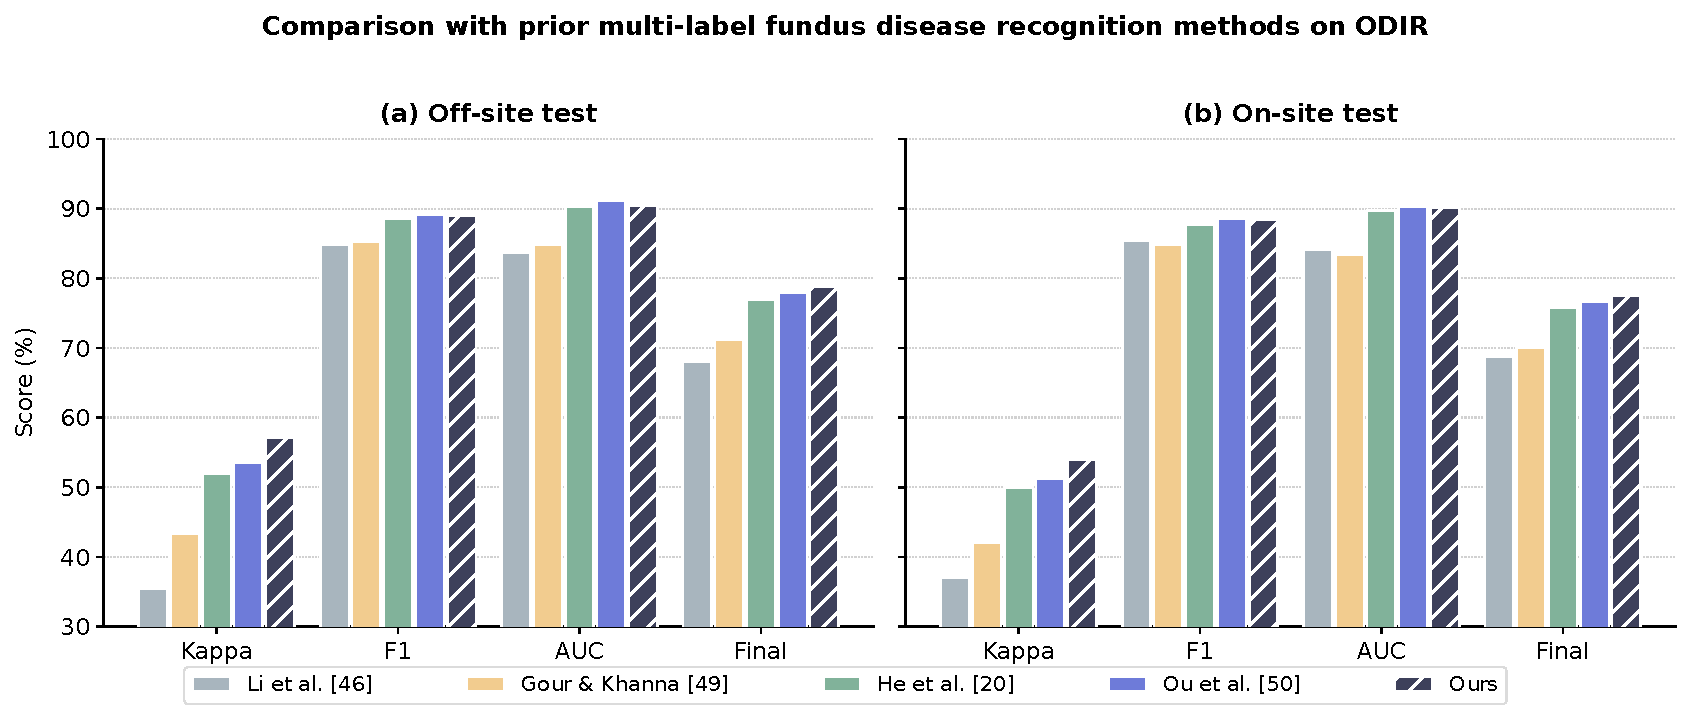
\includegraphics[width=0.96\textwidth]{images/plots/fig_sota_compare.pdf}
\caption{Visual comparison of metrics with existing methods on ODIR, where (a) Off-site test and (b) On-site test correspond to the two groups of binocular metrics in \hyperref[tab:sota-compare]{Table~\ref*{tab:sota-compare}}. The bars are grouped by the four metrics Kappa, F1, AUC, and Final score; within each metric, red values mark the best result and blue values mark the second-best. The proposed method (Ours) achieves the best Kappa and Final score on both test sets.}
\label{fig:sota-compare}
\end{figure}

The methods listed in Table 2 mainly focus on improving in-domain multi-label classification on ODIR. To address cross-institutional application needs and restrictions on medical data sharing, our framework extends multi-label recognition by incorporating single-source domain generalization and privacy protection. The proposed method achieves higher Final scores than the four compared methods on both ODIR Off-site and On-site. We also evaluate cross-dataset generalization on RFMiD and EDID under single-source training and examine classification performance under privacy-preserving training. These results suggest the framework’s potential for clinical ocular disease recognition where generalization and privacy protection are required.

\subsection{Ablation Study Results}

To assess the independent contributions and combined effects of the two core modules in the proposed method, namely Dual-Branch Guided Domain-Invariant Feature Extraction (DFE) and Adaptive Label-Feature Relevance Construction (ARC), and to examine the improvement in model interpretability brought by CAM guidance, we conduct module-wise ablation experiments using ODIR Off-site metrics. The results are shown in \hyperref[tab:ablation]{Table~\ref*{tab:ablation}}, and \hyperref[fig:ablation-radar]{Fig.~\ref*{fig:ablation-radar}} provides an intuitive radar-chart comparison of the metric distributions across models. \hyperref[tab:ablation]{Table~\ref*{tab:ablation}} reports both monocular and binocular metrics, which show a consistent improvement trend; to align with the official patient-level evaluation standard and keep the main text concise, the following analysis focuses on the binocular metrics.

% Chapter 4 Experiments - Table 3
% Ablation study of DFE and ARC modules.
\begin{table}
\centering
\caption{Ablation study results. The table reports monocular and binocular metrics on the ODIR Off-site test set. Compared with ResNet50 (baseline), introducing DFE or ARC alone and combining the two both yield performance improvements.}
\label{tab:ablation}
\resizebox{\textwidth}{!}{
\begin{tabular}{lcccccccc}
\toprule
\multirow{2}{*}{Model} & \multicolumn{4}{c}{Monocular} & \multicolumn{4}{c}{Binocular} \\
\cmidrule(lr){2-5}\cmidrule(lr){6-9}
& Kappa & F1 & AUC & Final & Kappa & F1 & AUC & Final \\
\midrule
ResNet50 & 58.52 & 90.18 & 89.40 & 79.37 & 52.75 & 87.83 & 88.00 & 76.19 \\
ResNet50+DFE & 62.09 & 91.04 & 91.64 & 81.59 & 56.20 & 88.80 & 90.10 & 78.37 \\
ResNet50+ARC & 59.41 & 90.14 & 91.74 & 80.43 & 53.19 & 87.45 & 90.29 & 76.98 \\
\textbf{ResNet50+DFE+ARC (Ours)} & \textbf{62.61} & \textbf{91.08} & \textbf{92.33} & \textbf{82.00} & \textbf{57.05} & \textbf{89.03} & \textbf{90.48} & \textbf{78.85} \\
\bottomrule
\end{tabular}
}
\end{table}


\begin{figure}
\centering
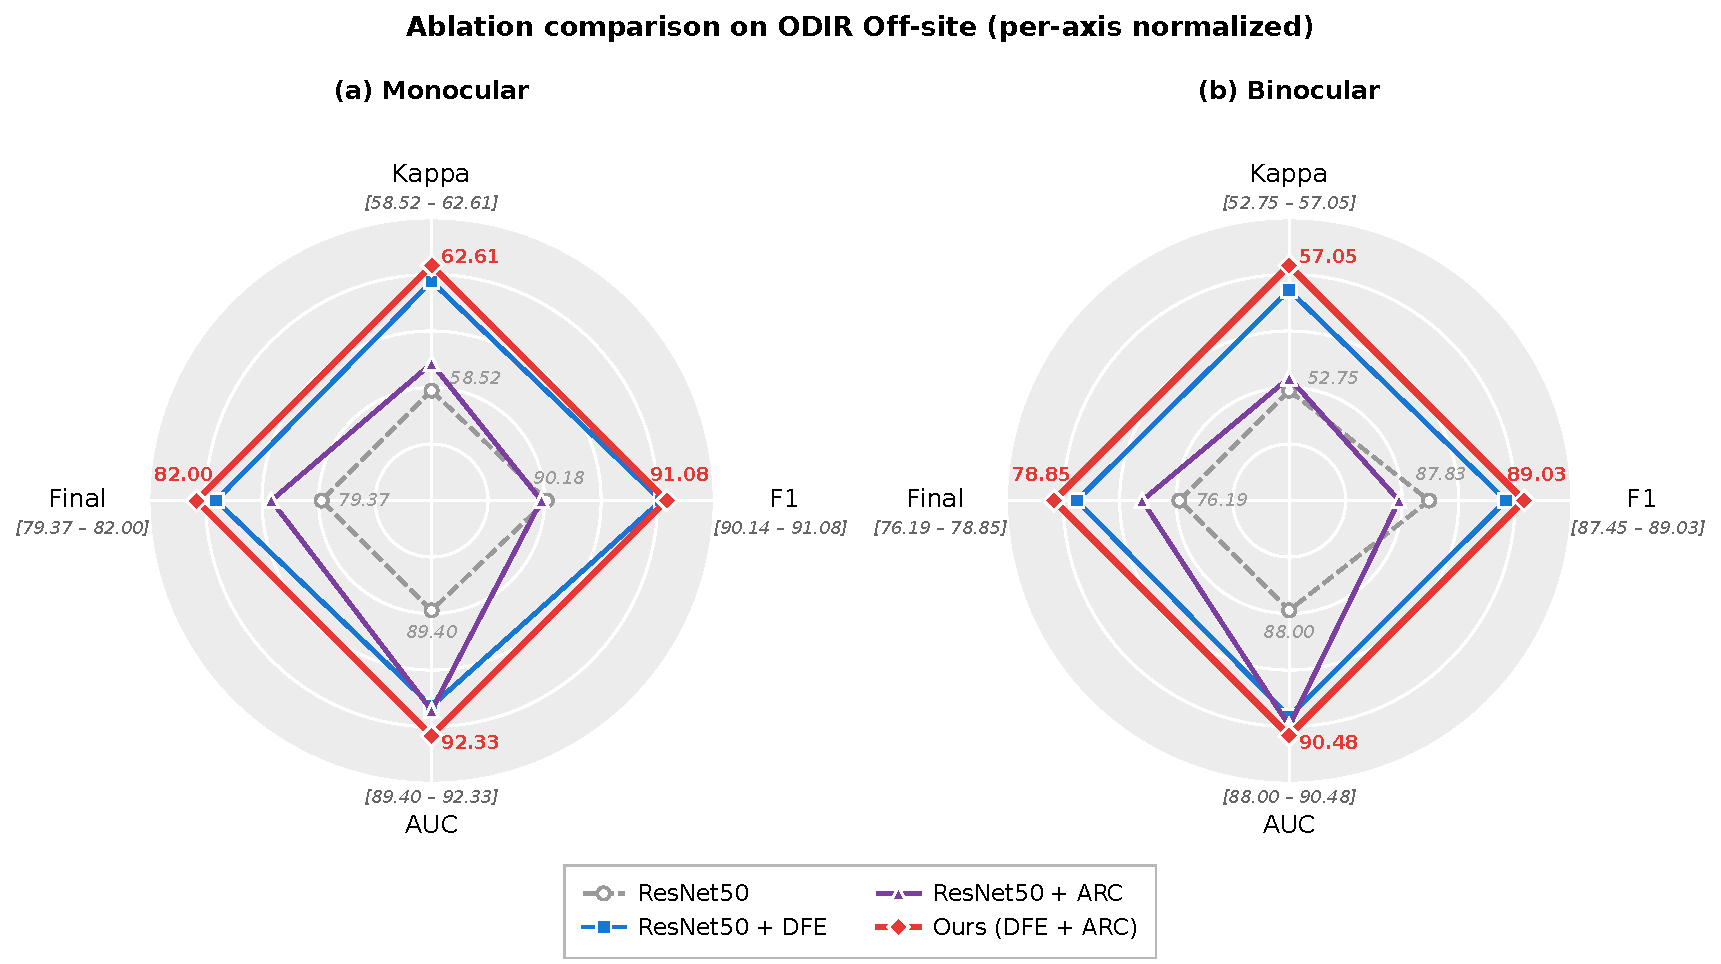
\includegraphics[width=0.92\textwidth]{images/plots/fig_ablation_radar.pdf}
\caption{Radar charts of the metrics of each model on ODIR Off-site in the ablation study, showing the results under (a) monocular and (b) binocular evaluation protocols, both consistent with \hyperref[tab:ablation]{Table~\ref*{tab:ablation}}. Each axis corresponds to one metric (Kappa, F1, AUC, Final) and is independently normalized according to the value range of that axis to amplify differences among models; the further the polygon extends outward, the higher the metric.}
\label{fig:ablation-radar}
\end{figure}

\begin{itemize}
\item

  ResNet50: only a single-branch ResNet50 and a standard multi-label classification head are used. The Final score is 76.19, Kappa is 52.75, and AUC is 88.00.
\item

  ResNet50+DFE: only the complete Dual-Branch Guided Domain-Invariant Feature Extraction module is introduced. The Final score increases to 78.37 (+2.18), Kappa increases by 3.45, and AUC increases by 2.10. The improvement mainly comes from CAM-guided residual weighting and the mask mechanism, which effectively suppress domain-specific noise and encourage the model to focus on domain-invariant features.

\item

  ResNet50+ARC: only the Adaptive Label-Feature Relevance Construction module is introduced. The Final score increases to 76.98 (+0.79), Kappa increases by 0.44, and AUC increases by 2.29. By explicitly modeling disease co-occurrence dependencies, such as DR and AMD or Myopia and optic-disc abnormalities, this module reduces the false-negative rate and improves multi-label recognition performance.
\item

  ResNet50+DFE+ARC (the proposed method, ours): when both modules are enabled, the Final score further increases to 78.85 (+2.66 over the baseline), Kappa reaches 57.05 (+4.30), and F1 and AUC reach 89.03 (+1.20) and 90.48 (+2.48), respectively. The combined model improves the Final score by 0.48 and 1.87 percentage points over the DFE-only and ARC-only configurations, respectively. These results show that each module contributes to performance improvement and that their combination achieves the best performance among the four configurations. DFE provides more stable domain-invariant features for ARC, enabling Transformer to learn label-label relevance and label-feature relevance more accurately. Conversely, the attention consistency loss of ARC further constrains the output distributions of the two branches and improves feature stability. In addition, the visualization results in \hyperref[fig:cam-visualization]{Fig.~\ref*{fig:cam-visualization}} show that, compared with the baseline, the CAMs obtained by the proposed method respond less to image edges and illumination artifacts, and the model-attended regions concentrate more on the eyeball, vessels, and other disease-related regions, indicating enhanced model interpretability.
\end{itemize}

\begin{figure}
\centering
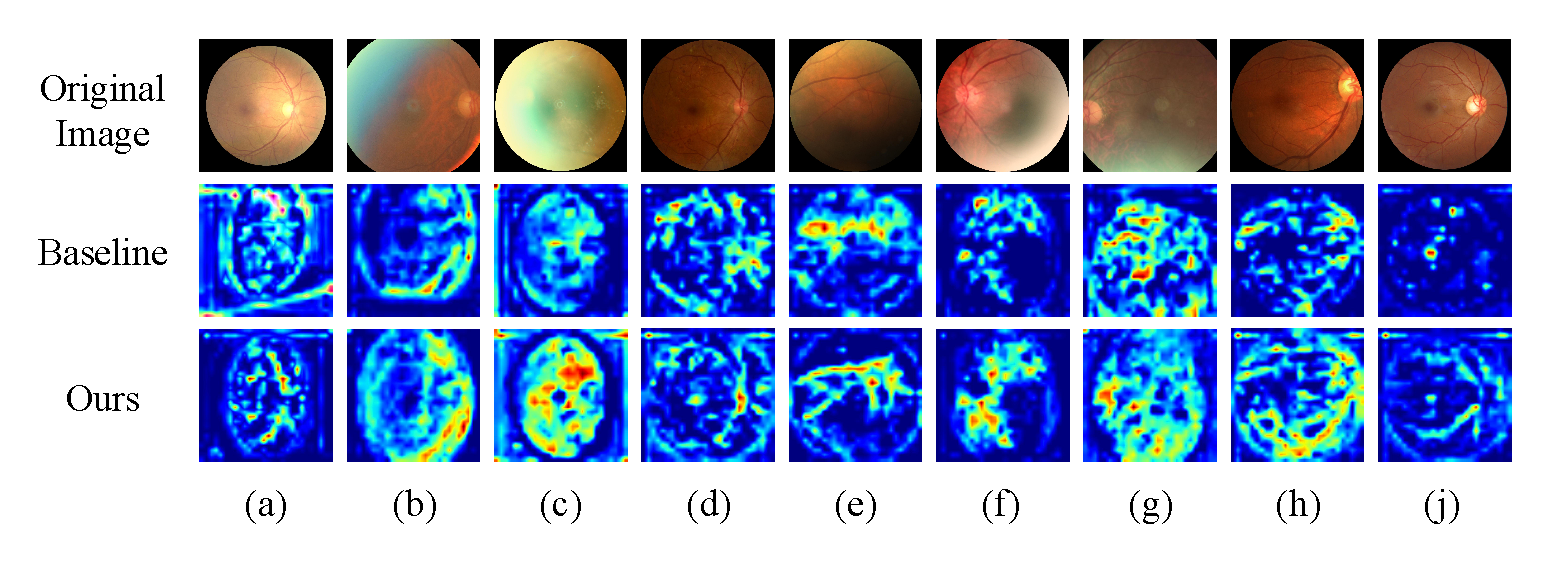
\includegraphics[width=0.92\textwidth]{images/media/image8_padded.pdf}
\caption{Comparison of CAM-based model-attended region visualizations between the baseline and the proposed method on selected ODIR Off-site samples, where (a)--(j) denote different test samples. Compared with the baseline, the model-attended regions of the proposed method are more concentrated on the eyeball, vessels, and disease-related regions, with weaker responses to irrelevant background factors such as image edges and illumination artifacts.}
\label{fig:cam-visualization}
\end{figure}

The ablation results show that Adaptive Label-Feature Relevance Construction (ARC) improves label relevance modeling in multi-disease co-occurrence scenarios, while Dual-Branch Guided Domain-Invariant Feature Extraction (DFE) supports learning domain-invariant features from a single source domain when multi-institutional joint training is restricted. The integration of the two modules further improves multi-label recognition performance under single-source-domain training and provides a basis for the subsequent cross-domain generalization results.

\subsection{Generalization Performance Results}

To comprehensively validate the generalization capability of the proposed method under single-source-domain training and the effectiveness of the privacy-preserving mechanism, we organize the evaluation in three stages: in-domain generalization, cross-domain generalization, and privacy preservation. We first validate multi-label recognition performance within the ODIR domain (Off-site and On-site), then examine cross-domain generalization capability on the two unseen domains RFMiD and EDID, and finally evaluate the performance retention after introducing the privacy-preserving mechanism. The first two stages are completed under the non-private setting, while the third stage is completed under the privacy-preserving setting.

1. Generalization performance under the non-private setting. The results are shown in \hyperref[tab:generalization]{Table~\ref*{tab:generalization}}, which reports the Final scores of the baseline and the proposed method on different test sets. The generalization experiments are organized along three evaluation directions: ODIR in-domain Off-site \(\rightarrow\) On-site, cross-domain generalization from ODIR to RFMiD, and cross-domain generalization from ODIR to EDID. For each direction, model selection and evaluation are based on the top five candidate checkpoints saved during training. Specifically, the checkpoint group with the best test-set performance is selected from the candidate checkpoints of the baseline and the proposed method, respectively, and the results of this checkpoint group on the source-domain Off-site set and the target domain are reported simultaneously.

% Chapter 4 Experiments - Table 4
% Generalization performance on ODIR, RFMiD/RIADD, and EDID.
\begin{table}
\centering
\caption{Comparison of generalization performance on different test sets. The table compares the baseline and the proposed method on ODIR in-domain generalization (Off-site $\rightarrow$ On-site) and cross-domain generalization from ODIR to RFMiD and EDID, using Final score as the metric. Off-site $\rightarrow$ On-site reports both monocular and binocular results, while cross-domain generalization reports monocular results after aligning each dataset to a three-class label space. For each direction, the checkpoint with the best test-set performance is selected from candidate checkpoints.}
\label{tab:generalization}
\resizebox{\textwidth}{!}{
\begin{tabular}{lcccccccc}
\toprule
\multirow{3}{*}{Model} & \multicolumn{4}{c}{Off-site $\rightarrow$ On-site} & \multicolumn{2}{c}{Off-site $\rightarrow$ RFMiD} & \multicolumn{2}{c}{Off-site $\rightarrow$ EDID} \\
\cmidrule(lr){2-5}\cmidrule(lr){6-7}\cmidrule(lr){8-9}
& \multicolumn{2}{c}{Off-site} & \multicolumn{2}{c}{On-site} & Off-site & RFMiD & Off-site & EDID \\
\cmidrule(lr){2-3}\cmidrule(lr){4-5}\cmidrule(lr){6-7}\cmidrule(lr){8-9}
& Monocular & Binocular & Monocular & Binocular & Monocular & Monocular & Monocular & Monocular \\
\midrule
ResNet50 & 79.37 & 76.19 & 77.30 & 75.23 & 94.39 & 83.86 & 94.30 & 52.16 \\
\textbf{Ours} & \textbf{81.71} & \textbf{78.79} & \textbf{78.98} & \textbf{77.49} & \textbf{95.94} & \textbf{85.06} & \textbf{96.03} & \textbf{55.35} \\
\bottomrule
\end{tabular}
}
\end{table}


For ODIR in-domain generalization, the test set is On-site, and \hyperref[tab:generalization]{Table~\ref*{tab:generalization}} reports both monocular and binocular evaluation protocols. The baseline checkpoint achieves binocular scores of 76.19 and 75.23 on Off-site and On-site, respectively, whereas the corresponding checkpoint of the proposed method improves these scores to 78.79 and 77.49, with gains of 2.60 and 2.26 percentage points. The monocular metrics also increase from 79.37 and 77.30 to 81.71 and 78.98. This indicates that dual-branch guided feature learning and CAM-guided attention can enhance the model's focus on disease-related regions. Binocular metrics are lower than monocular metrics because the model is trained with monocular data. During inference, when the left-eye and right-eye predictions of the same patient are merged, an incorrect prediction from either eye may affect patient-level judgment, amplifying the effect of small monocular errors on the final metric.

For cross-domain generalization, the complete label spaces of RFMiD, EDID, and ODIR are inconsistent. Therefore, this study first reconstructs shared three-class label spaces before generalization evaluation. RFMiD is aligned using D/A/M classes, while EDID is aligned using D/G/M classes. Although EDID is a single-label dataset, it can still be used as a cross-domain generalization dataset under the three-class shared label space. Considering that the cross-domain generalization datasets differ more significantly from ODIR in imaging devices, acquisition procedures, illumination conditions, disease composition, and label definitions, model selection and evaluation are also based on the top five candidate checkpoints. The monocular Final scores of the selected checkpoint group on the three-class ODIR Off-site set and the cross-domain generalization dataset are reported simultaneously.

In RFMiD D/A/M cross-domain generalization, the baseline checkpoint obtains a Final score of 94.39 on ODIR Off-site and 83.86 on the target domain. The corresponding checkpoint of the proposed method obtains a Final score of 95.94 on ODIR Off-site and 85.06 on the target domain, improving by 1.55 and 1.20 percentage points, respectively. Detailed metrics show that the Kappa, F1, and AUC of the proposed method on RFMiD are 73.95, 87.96, and 93.27, all higher than the baseline values of 72.08, 87.11, and 92.39. In EDID D/G/M cross-domain generalization, the baseline checkpoint obtains a Final score of 94.30 on ODIR Off-site and 52.16 on the target domain. The proposed method obtains 96.03 on ODIR Off-site and 55.35 on the target domain, improving by 1.73 and 3.19 percentage points, respectively. The Kappa, F1, and AUC of the proposed method on EDID are 27.20, 67.22, and 71.63, which are higher than the baseline values of 23.83, 65.54, and 67.09. Overall, the RFMiD results validate the cross-domain generalization capability of the model on a multi-label dataset, while the EDID results further indicate that the proposed method remains effective when a single-label dataset is incorporated into a three-class generalization evaluation framework. \hyperref[fig:tsne]{Fig.~\ref*{fig:tsne}} further visualizes the target-domain feature distributions under selected evaluation directions using t-SNE. In the ODIR in-domain direction (\figsubref{fig:tsne}{a}), Off-site and On-site share the same source and the domain gap itself is small, so same-class samples of both methods overlap reasonably, while Ours shows clearer local cluster structures on the small-sample disease classes (G, A, M). In the RFMiD cross-domain direction (\figsubref{fig:tsne}{b}), Ours organizes the D/A/M classes into more independent clusters, with source- and target-domain samples of the same class closely mixed within each cluster, whereas the baseline has multiple separated sub-clusters within class D and looser local aggregation of the three classes.

\begin{figure}
\centering
\begin{subfigure}{\textwidth}
\centering
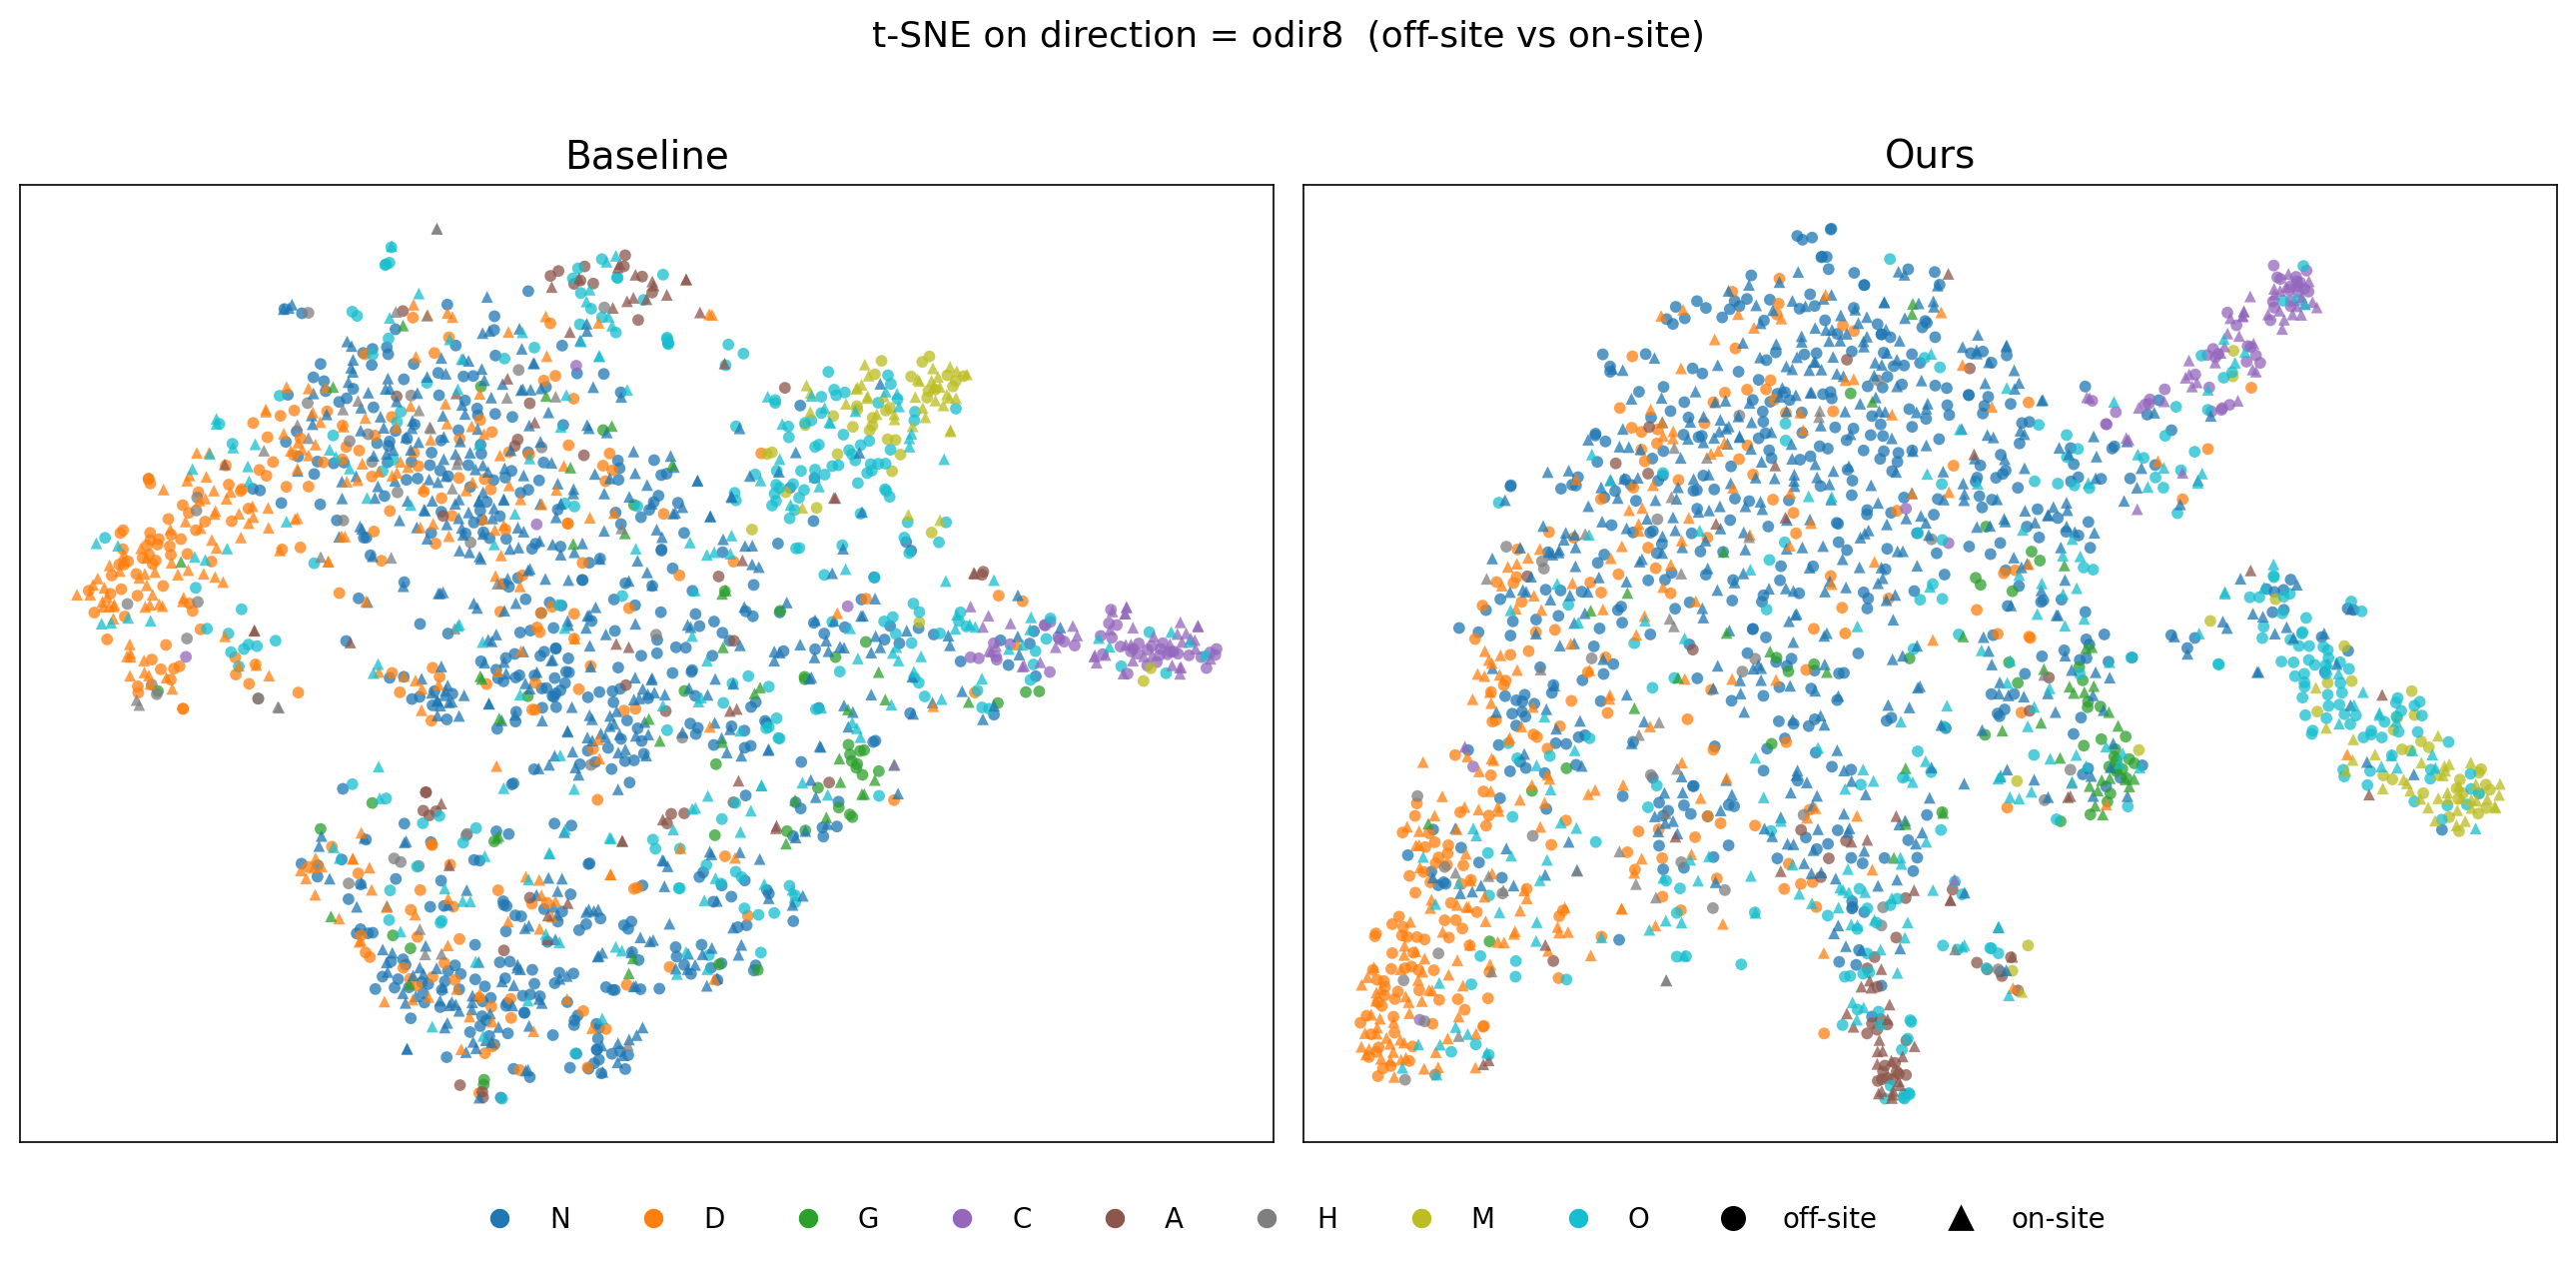
\includegraphics[width=0.60\textwidth]{images/plots/tsne_odir8_panel1_tx.png}
\caption{ODIR Off-site \(\rightarrow\) On-site (in-domain generalization, 8 classes)}
\label{fig:tsne-odir}
\end{subfigure}

\vspace{4pt}
\begin{subfigure}{\textwidth}
\centering
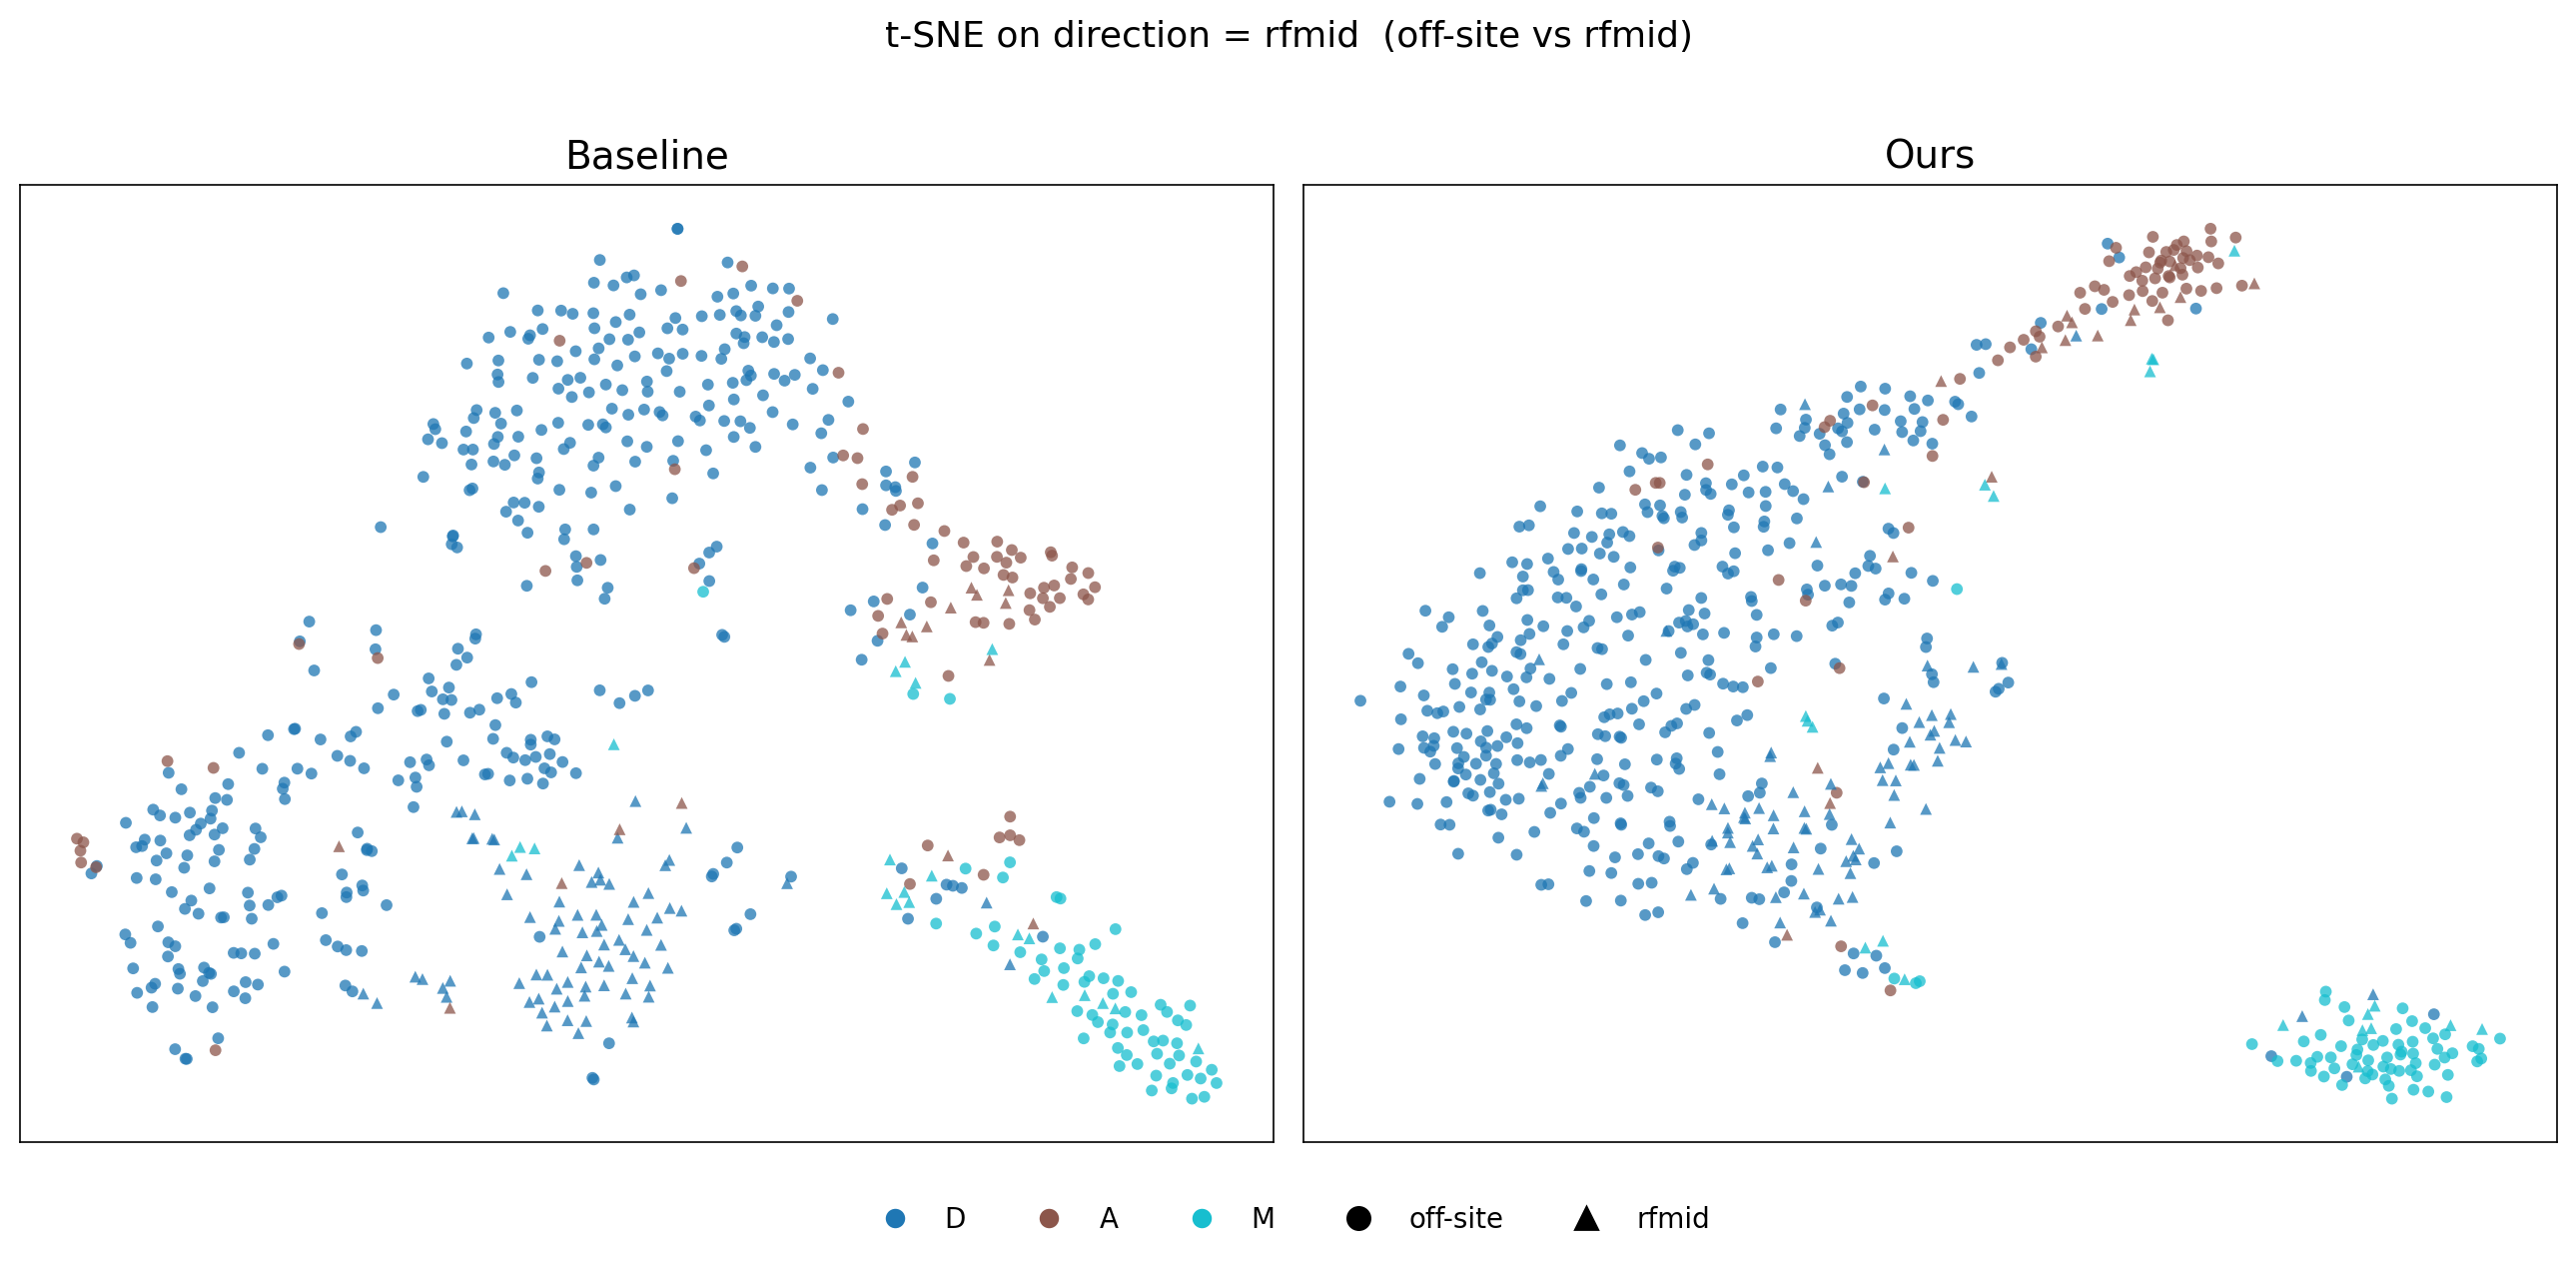
\includegraphics[width=0.60\textwidth]{images/plots/tsne_rfmid_panel1_tx.png}
\caption{ODIR Off-site \(\rightarrow\) RFMiD (D/A/M three-class alignment)}
\label{fig:tsne-rfmid}
\end{subfigure}
\captionsetup{font=small}
\caption{t-SNE visualization of target-domain sample features under selected evaluation directions, where (a)--(b) correspond to ODIR in-domain (Off-site \(\rightarrow\) On-site) and ODIR \(\rightarrow\) RFMiD, respectively. In each subfigure, the left side is the baseline and the right side is the proposed method (Ours); different colors denote different classes, dots denote source-domain samples, and triangles denote target-domain samples.}
\label{fig:tsne}
\end{figure}

\begin{sloppypar}
2. Hyperparameter scan of Adaptive Gaussian Differential Privacy. The results are shown in \hyperref[tab:privacy-scan]{Table~\ref*{tab:privacy-scan}}. After introducing privacy preservation, the noise injection rate affects model convergence behavior and final performance. The experiments show that the noise multiplier and noise decay rate jointly determine the per-epoch noise injection rate and further affect privacy budget consumption in each epoch. Excessive initial noise causes severe training oscillation or even non-convergence, whereas overly fast decay exhausts the privacy budget before the model has learned sufficiently. Setting 1 (noise\_multiplier=0.65) provides very strong privacy preservation, but the excessive initial noise yields \(\epsilon=5.01\) and severely degrades model performance. Setting 8 (noise\_multiplier=0.25, noise\_decay\_rate=4e\mbox{-}6) brings model performance close to the non-private setting, but \(\epsilon \approx 20\) indicates weak privacy preservation. Considering both performance and privacy budget, we finally select Setting 5 (noise\_multiplier=0.35, noise\_decay\_rate=4e\mbox{-}6), which reaches \(\epsilon \approx 10.15\) after 80 epochs and achieves a better privacy-performance trade-off.
\end{sloppypar}

% Chapter 4 Experiments - Table 5
% Hyperparameter scan for adaptive Gaussian differential privacy.
\begin{table}
\centering
\caption{Hyperparameter scan results for Adaptive Gaussian Differential Privacy. The table compares the privacy budget $\epsilon$ under 80-epoch differential privacy training with different combinations of noise multiplier and noise decay rate. The red Setting 5 is the final setting used in this study.}
\label{tab:privacy-scan}
\begin{tabular}{lccc}
\toprule
Setting & noise\_multiplier & noise\_decay\_rate & $\epsilon$ / 80 epoch \\
\midrule
setting1 & 0.65 & 1.5e-6 & 5.01 \\
setting2 & 0.50 & 2e-6 & 6.80 \\
setting3 & 0.40 & 4e-6 & 8.71 \\
setting4 & 0.35 & 2e-6 & 9.96 \\
\textcolor{red}{setting5} & \textcolor{red}{0.35} & \textcolor{red}{4e-6} & \textcolor{red}{10.15} \\
setting6 & 0.30 & 2e-6 & 11.91 \\
setting7 & 0.25 & 2e-6 & 15.11 \\
setting8 & 0.25 & 4e-6 & 20.01 \\
\bottomrule
\end{tabular}
\end{table}


3. \(\epsilon\)-performance evolution and optimization strategy during privacy-preserving training. The results are shown in \hyperref[tab:privacy-evolution]{Table~\ref*{tab:privacy-evolution}} and are intuitively presented as a privacy-performance trade-off curve in \hyperref[fig:privacy-tradeoff]{Fig.~\ref*{fig:privacy-tradeoff}}. After adopting the noise rate of Setting 5, we record epoch-by-epoch changes in \(\epsilon\) consumption and monocular metrics during training. As \(\epsilon\) increases from 0.94 at epoch 0 to 10.15 at epoch 79, the privacy budget is progressively spent and model performance improves, reaching a peak around epoch 74 (Final=73.15). This indicates that the adaptive decay strategy allows the model to learn sufficiently within the privacy budget. The checkpoint at epoch 74 provides the best balance between privacy preservation and performance. Extensive experiments show that the optimization strategy needs to be adjusted for privacy-preserving scenarios:

% Chapter 4 Experiments - Table 6
% Epsilon-performance evolution during privacy training.
\begin{table}
\centering
\caption{Evolution of $\epsilon$ and performance during privacy-preserving training. The table uses the noise injection strategy of Setting 5 in \tabref{tab:privacy-scan}, and the evaluation metric is monocular Final score. As training proceeds, the privacy budget is progressively spent and model performance generally increases, reaching its peak at e74 (red). This checkpoint is used as the optimal privacy checkpoint under privacy preservation in this study.}
\label{tab:privacy-evolution}
\begin{tabular}{lccccc}
\toprule
Epoch & $\epsilon$ & Kappa & F1 & AUC & Final \\
\midrule
e0 & 0.94 & 29.39 & 84.70 & 78.70 & 64.26 \\
e10 & 3.28 & 34.24 & 85.77 & 81.27 & 67.09 \\
e22 & 4.91 & 36.42 & 85.85 & 82.83 & 68.36 \\
e31 & 5.91 & 39.70 & 86.28 & 83.56 & 69.85 \\
e40 & 6.81 & 40.62 & 86.13 & 84.08 & 70.28 \\
e49 & 7.65 & 40.64 & 87.01 & 85.17 & 70.94 \\
e52 & 7.92 & 42.16 & 87.46 & 85.00 & 71.54 \\
e64 & 8.94 & 42.45 & 87.38 & 85.89 & 71.91 \\
e68 & 9.27 & 43.59 & 87.76 & 86.18 & 72.51 \\
\textcolor{red}{e74} & \textcolor{red}{9.76} & \textcolor{red}{45.12} & \textcolor{red}{87.91} & \textcolor{red}{86.42} & \textcolor{red}{73.15} \\
e79 & 10.15 & 43.16 & 87.51 & 86.47 & 72.38 \\
\bottomrule
\end{tabular}
\end{table}


\begin{figure}
\centering
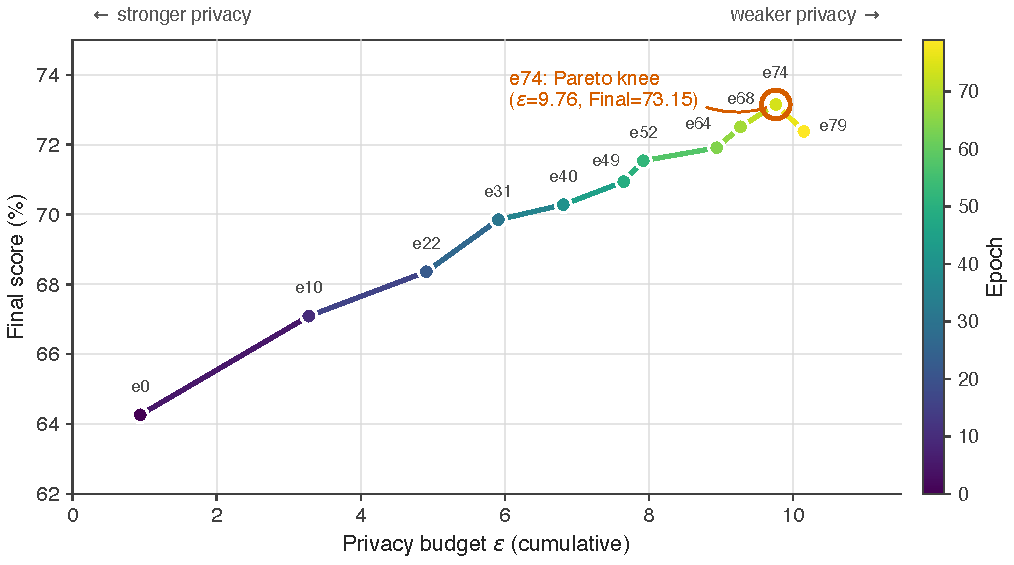
\includegraphics[width=0.78\textwidth]{images/plots/fig_privacy_tradeoff.pdf}
\caption{Privacy-performance (\(\epsilon\)-Final score) trade-off curve during privacy-preserving training, with data corresponding to \hyperref[tab:privacy-evolution]{Table~\ref*{tab:privacy-evolution}}. The horizontal axis is the cumulative privacy budget \(\epsilon\) (stronger privacy preservation toward the left), and the vertical axis is the monocular Final score. Each point corresponds to an epoch checkpoint and is colored by training epoch; the trajectory shows the privacy-performance evolution as training proceeds. Epoch 74 (e74) is the Pareto knee point, achieving the best Final score (73.15) at \(\epsilon \approx 9.76\), and is the best operating point that balances privacy and performance.}
\label{fig:privacy-tradeoff}
\end{figure}

(1) The learning rate is increased from \(1 \times 10^{-5}\) to \(7.5 \times 10^{-5}\).

(2) The learning-rate schedule is changed to linear decay followed by constant training. The learning rate decay ratio and final learning rate factor control the decay epochs and decay ratio, and are set to 0.75 and 0.8, respectively. That is, the learning rate linearly decays to 80\% of its original value during the first 75\% of epochs and then remains constant.

This adjustment is motivated by the differences between privacy-preserving training and non-private training. For the learning rate, noise is added to each backpropagated gradient under privacy-preserving training, causing the loss at each optimization step to fluctuate and increasing the risk of poor local optima. A moderately larger learning rate is therefore needed. For the learning-rate schedule, non-private training usually decreases the learning rate as the model approaches an optimum. In contrast, privacy-preserving training does not need to reduce the learning rate to a very small value, because differential privacy training continues optimization while privacy loss accumulates, but may not fully converge. Starting with a relatively large learning rate, linearly decaying it to a smaller value over a certain period, and then keeping it constant therefore yields better performance.

Experiments demonstrate that this strategy improves convergence stability and achieves a Final score of 73.15 at \(\epsilon = 9.76\), clearly outperforming fixed-noise or low-learning-rate configurations.

4. Final generalization performance under privacy preservation. The results are shown in \hyperref[tab:privacy-final]{Table~\ref*{tab:privacy-final}}. Since existing generalization studies on multi-label ocular disease recognition rarely report metrics under privacy-preserving training, this study uses the official ODIR ResNet50 baseline provided by Li et al. \cite{_Ref213949402} as a public reference point to assess whether privacy-preserving training can maintain performance comparable to a public benchmark. Under their respective training configurations, our non-private and private models achieve Off-site Final scores of 78.85 and 68.96, and On-site Final scores of 77.49 and 68.42, respectively. The differences of 9.89 and 9.07 percentage points quantify the recognition performance cost associated with privacy-preserving training. Compared with the official baseline, the proposed method is slightly better on Off-site (68.96 vs. 68.00) and slightly lower on On-site (68.42 vs. 68.80), remaining around the public benchmark overall. This indicates that, under a moderate privacy budget, the Adaptive Gaussian Differential Privacy mechanism can provide effective privacy preservation while keeping performance within an acceptable range.
% Chapter 4 Experiments - Table 7
% Final generalization performance under privacy mode.
\begin{table}
\centering
\caption{Comparison of generalization performance under privacy preservation. The table reports ODIR in-domain binocular Final score. Ours (privacy) uses the optimal privacy checkpoint selected in \tabref{tab:privacy-evolution}, with the official baseline reported by Li et al. \cite{_Ref213949402} as a public reference.}
\label{tab:privacy-final}
\begin{tabular}{lcc}
\toprule
Model & Off-site & On-site \\
\midrule
Li et al. \cite{_Ref213949402} & 68.00 & \textbf{68.80} \\
\textbf{Ours (privacy)} & \textbf{68.96} & 68.42 \\
\bottomrule
\end{tabular}
\end{table}


\FloatBarrier

\section{Conclusion and Discussion}

We propose a Privacy-Preserving Interpretable Single-Domain Generalization framework for multi-label ocular disease recognition. The framework provides a unified solution to a set of progressive challenges: clinical multi-disease co-occurrence, cross-institutional domain shift, and the privacy sensitivity that further restricts multi-source collaboration. The core contributions are as follows: (1) the Adaptive Label-Feature Relevance Construction (ARC) module uses Transformer self-attention and cross-attention mechanisms to capture label-label relevance and label-feature relevance, and aligns dual-branch outputs through attention consistency loss, helping reduce false positives and false negatives in multi-label recognition; (2) the Dual-Branch Guided Domain-Invariant Feature Extraction (DFE) module simulates potential domain shift through style augmentation, uses CAM to provide disease-region prior guidance, and combines spatial/channel attention with a dual-branch mask-based contrastive learning mechanism to extract domain-invariant features, improving unseen-domain generalization performance while enhancing model interpretability; and (3) the Adaptive Gaussian Differential Privacy (AdaGDP) mechanism dynamically decays noise intensity to achieve a balance between privacy preservation and model performance under a moderate privacy budget (\(\epsilon \approx 10\)). Systematic experiments validate the effectiveness of the proposed method. Despite these advances, the framework still has limitations. Class imbalance may affect the stability of recognition for minority disease classes, which could be further alleviated by resampling or loss weighting in future work. In addition, current cross-domain generalization is mainly based on shared label spaces, and future work can explore generalization under open-category and more complex out-of-distribution scenarios. Furthermore, in terms of privacy preservation, future work can explore methods that retain performance under tighter privacy budgets, or combine the proposed mechanism with federated learning and similar techniques to adapt to more complex cross-institutional deployment scenarios.


\begin{thebibliography}{50}
\bibitem{_Ref213949315}
Zhang W, Zhao X, Chen Y, et al. DeepUWF: an automated ultra-wide-field fundus screening system via deep learning. IEEE Journal of Biomedical and Health Informatics 2020;25(8): 2988-2996.
\bibitem{_RefRahman2022MLFundus}
Mujeeb Rahman K K, Nasor M, Imran A. Automatic screening of diabetic retinopathy using fundus images and machine learning algorithms. Diagnostics 2022;12(9): 2262.
\bibitem{_RefLim2024VLVOphthalmology}
Lim G, Elangovan K, Jin L. Vision language models in ophthalmology. Current Opinion in Ophthalmology 2024;35(6): 487-493.
\bibitem{_RefUrooj2025LLMMedicalImage}
Urooj B, Fayaz M, Ali S, et al. Large language models in medical image analysis: a systematic survey and future directions. Bioengineering 2025;12(8): 818.
\bibitem{_Ref213871637}
Kumar V, Singh R S, Rambabu M, et al. Deep learning for hyperspectral image classification: A survey. Computer Science Review 2024;53: 100658.
\bibitem{_Ref213948625}
Mo Y, Wu Y, Yang X, et al. Review the state-of-the-art technologies of semantic segmentation based on deep learning. Neurocomputing 2022;493: 626-646.
\bibitem{_Ref213948898}
Qiu D, Cheng Y, Wang X. Medical image super-resolution reconstruction algorithms based on deep learning: A survey. Computer Methods and Programs in Biomedicine 2023;238: 107590.
\bibitem{_Ref213949262}
Hasan S M M, Uddin M P, Al Mamun M, et al. A machine learning framework for early-stage detection of autism spectrum disorders. IEEE Access 2022;11: 15038-15057.
\bibitem{_Ref213949362}
Al-Fahdawi S, Al-Waisy A S, Zeebaree D Q, et al. Fundus-deepnet: Multi-label deep learning classification system for enhanced detection of multiple ocular diseases through data fusion of fundus images. Information Fusion 2024;102: 102059.
\bibitem{_Ref213949382}
Chen Z M, Wei X S, Wang P, et al. Multi-label image recognition with graph convolutional networks. In: Proceedings of the IEEE/CVF conference on computer vision and pattern recognition; 2019. p. 5177-5186.
\bibitem{_Ref213949348}
Liu S, Yin S, Qu L, et al. Reducing domain gap in frequency and spatial domain for cross-modality domain adaptation on medical image segmentation. In: Proceedings of the AAAI conference on artificial intelligence; 2023;37(2): 1719-1727.
\bibitem{_Ref213949354}
Yang C, Guo X, Chen Z, et al. Source free domain adaptation for medical image segmentation with fourier style mining. Medical Image Analysis 2022;79: 102457.
\bibitem{_Ref213949393}
Bertino E, Ooi B C, Yang Y, et al. Privacy and ownership preserving of outsourced medical data. In: 21st International Conference on Data Engineering (ICDE\textquotesingle05). IEEE; 2005. p. 521-532.
\bibitem{_Ref213949872}
Wang Y, Xie Y, Fan L, et al. STMG: Swin transformer for multi-label image recognition with graph convolution network. Neural Computing and Applications 2022;34(12): 10051-10063.
\bibitem{_Ref213949896}
Zhang M L, Li Y K, Liu X Y, et al. Binary relevance for multi-label learning: an overview. Frontiers of Computer Science 2018;12(2): 191-202.
\bibitem{_Ref213949927}
Ridnik T, Ben-Baruch E, Zamir N, et al. Asymmetric loss for multi-label classification. In: Proceedings of the IEEE/CVF international conference on computer vision; 2021. p. 82-91.
\bibitem{_Ref213950246}
Liu S, Zhang L, Yang X, et al. Query2label: A simple transformer way to multi-label classification. arXiv preprint arXiv:2107.10834. 2021.
\bibitem{_Ref213950282}
Everingham M, Van Gool L, Williams C K I, et al. The pascal visual object classes (voc) challenge. International journal of computer vision 2010;88(2): 303-338.
\bibitem{_Ref213950349}
Cheng Y, Ma M, Li X, et al. Multi-label classification of fundus images based on graph convolutional network. BMC Medical Informatics and Decision Making 2021;21(Suppl 2): 82.
\bibitem{_Ref213950338}
He J, Li C, Ye J, et al. Multi-label ocular disease classification with a dense correlation deep neural network. Biomedical Signal Processing and Control 2021;63: 102167.
\bibitem{_Ref213950343}
Bhati A, Gour N, Khanna P, et al. Discriminative kernel convolution network for multi-label ophthalmic disease detection on imbalanced fundus image dataset. Computers in Biology and Medicine 2023;153: 106519.
\bibitem{_Ref213949439}
Guan H, Liu M. Domain adaptation for medical image analysis: a survey. IEEE Transactions on Biomedical Engineering 2021;69(3): 1173-1185.
\bibitem{_Ref213949448}
Tzeng E, Hoffman J, Zhang N, et al. Deep domain confusion: Maximizing for domain invariance. arXiv preprint arXiv:1412.3474. 2014.
\bibitem{_Ref213949453}
Sun B, Feng J, Saenko K. Return of frustratingly easy domain adaptation. In: \allowbreak Proceedings of the AAAI conference on artificial intelligence; 2016;30(1).
\bibitem{_Ref213949479}
Ganin Y, Ustinova E, Ajakan H, et al. Domain-adversarial training of neural networks. Journal of machine learning research 2016;17(59): 1-35.
\bibitem{_Ref213949490}
Zhu J Y, Park T, Isola P, et al. Unpaired image-to-image translation using cycle-consistent adversarial networks. In: Proceedings of the IEEE international conference on computer vision; 2017. p. 2223-2232.
\bibitem{_Ref213949530}
Wang R, Wu Z, Weng Z, et al. Cross-domain contrastive learning for unsupervised domain adaptation. IEEE Transactions on Multimedia 2022;25: 1665-1673.
\bibitem{_Ref213949554}
Zhou K, Liu Z, Qiao Y, et al. Domain generalization: A survey. IEEE transactions on pattern analysis and machine intelligence 2022;45(4): 4396-4415.
\bibitem{_Ref213949562}
Zhou K, Yang Y, Qiao Y, et al. Domain generalization with mixstyle. arXiv preprint arXiv:2104.02008. 2021.
\bibitem{_Ref213949607}
Gulrajani I, Lopez-Paz D. In search of lost domain generalization. arXiv preprint arXiv:2007.01434. 2020.
\bibitem{_Ref213949788}
Xu Q, Zhang R, Zhang Y, et al. A fourier-based framework for domain generalization. In: Proceedings of the IEEE/CVF conference on computer vision and pattern recognition; 2021. p. 14383-14392.
\bibitem{_Ref213949796}
Huang Z, Wang H, Xing E P, et al. Self-challenging improves cross-domain generalization. In: European conference on computer vision. Cham: Springer International Publishing; 2020. p. 124-140.
\bibitem{_Ref213949803}
Khoee A G, Yu Y, Feldt R. Domain generalization through meta-learning: a survey. Artificial Intelligence Review 2024;57(10): 285.
\bibitem{_Ref213949863}
Ouyang C, Chen C, Li S, et al. Causality-inspired single-source domain generalization for medical image segmentation. IEEE Transactions on Medical Imaging 2022;42(4): 1095-1106.
\bibitem{_Ref213950358}
Yadav N, Pandey S, Gupta A, et al. Data privacy in healthcare: in the era of artificial intelligence. Indian Dermatology Online Journal 2023;14(6): 788-792.
\bibitem{_Ref213950376}
Aledhari M, Razzak R, Parizi R M, et al. Federated learning: A survey on enabling technologies, protocols, and applications. IEEE Access 2020;8: 140699-140725.
\bibitem{_Ref213950391}
Li T, Sahu A K, Zaheer M, et al. Federated optimization in heterogeneous networks. Proceedings of Machine learning and systems 2020;2: 429-450.
\bibitem{_Ref213950427}
Martins P, Sousa L, Mariano A. A survey on fully homomorphic encryption: An engineering perspective. ACM Computing Surveys (CSUR) 2017;50(6): 1-33.
\bibitem{_Ref213950433}
Dutil F, See A, Di Jorio L, et al. Application of homomorphic encryption in medical imaging. arXiv preprint arXiv:2110.07768. 2021.
\bibitem{_Ref213950438}
Zhao C, Zhao S, Zhao M, et al. Secure multi-party computation: theory, practice and applications. Information Sciences 2019;476: 357-372.
\bibitem{_Ref213950443}
Bu Z, Dong J, Long Q, et al. Deep learning with gaussian differential privacy. Harvard data science review 2020;2020(23): 10.1162/99608f92.cfc5dd25.
\bibitem{_Ref213950449}
Dong J, Roth A, Su W J. Gaussian differential privacy. Journal of the Royal Statistical Society Series B: Statistical Methodology 2022;84(1): 3-37.
\bibitem{_Ref213950458}
Bagdasaryan E, Poursaeed O, Shmatikov V. Differential privacy has disparate impact on model accuracy. Advances in neural information processing systems 2019;32.
\bibitem{_RefResNet2016}
He K, Zhang X, Ren S, et al. Deep residual learning for image recognition. In: Proceedings of the IEEE conference on computer vision and pattern recognition; 2016. p. 770-778.
\bibitem{_Ref214903493}
Dwork C, McSherry F, Nissim K, et al. Calibrating noise to sensitivity in private data analysis. In: Theory of cryptography conference. Berlin, Heidelberg: Springer Berlin Heidelberg, 2006: 265-284.
\bibitem{_Ref213949402}
Li N, Li T, Hu C, et al. A benchmark of ocular disease intelligent recognition: One shot for multi-disease detection. In: International symposium on benchmarking, measuring and optimization. Cham: Springer International Publishing; 2020. p. 177-193.
\bibitem{_Ref213949409}
Pachade S, Porwal P, Thulkar D, et al. Retinal fundus multi-disease image dataset (rfmid): A dataset for multi-disease detection research. Data 2021;6(2): 14.
\bibitem{_RefEDID2024}
Sharmin S, Rashid M R, Khatun T, et al. A dataset of color fundus images for the detection and classification of eye diseases. Data in Brief 2024;57: 110979.
\bibitem{_Ref214903299}
Gour N, Khanna P. Multi-class multi-label ophthalmological disease detection using transfer learning based convolutional neural network. Biomedical signal processing and control 2021;66: 102329.
\bibitem{_Ref214903327}
Ou X, Gao L, Quan X, et al. BFENet: A two-stream interaction CNN method for multi-label ophthalmic diseases classification with bilateral fundus images. Computer Methods and Programs in Biomedicine 2022;219: 106739.
\end{thebibliography}


\end{document}
